\documentclass[letterpaper]{book}
\usepackage{graphicx}
\usepackage{wallpaper}
\usepackage{pdfpages}
\usepackage[utf8x]{inputenc}
\setcounter{secnumdepth}{-1}
\pagestyle{plain}

\begin{document}
\frontmatter
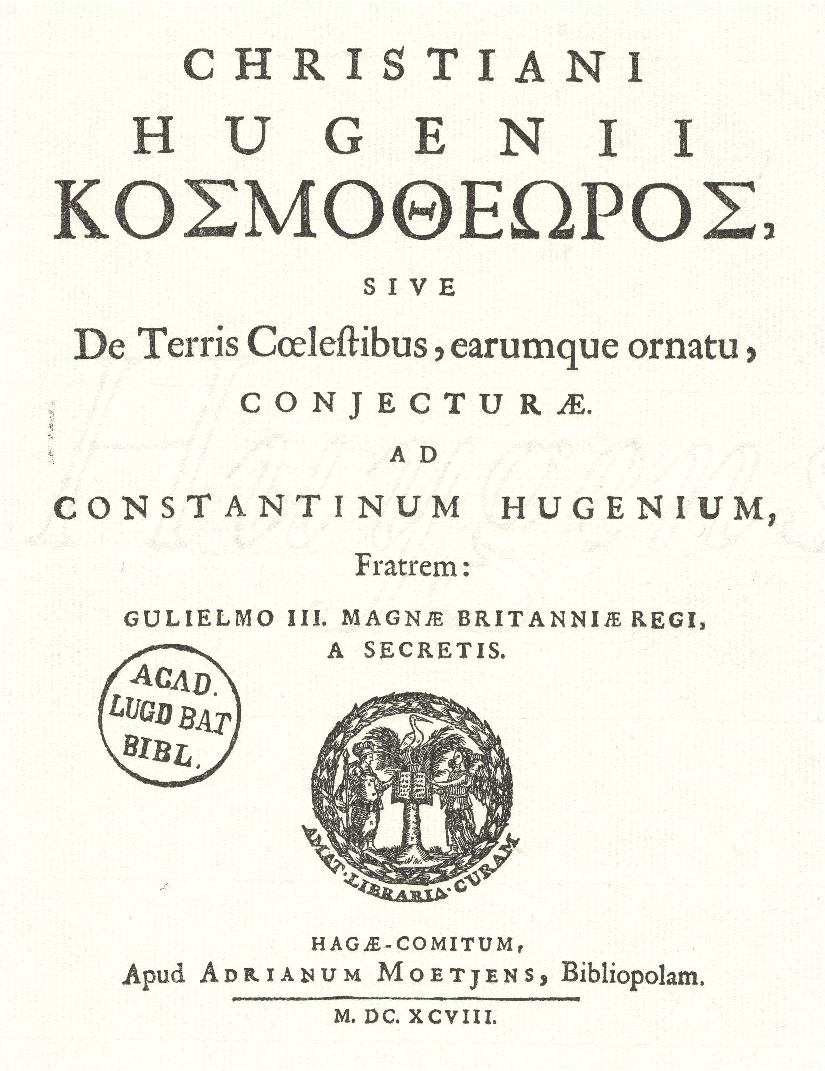
\includepdf{ct_title_la.pdf}
\thispagestyle{empty}

\begin{titlepage}
	\begin{center}
		\Huge
THE \\
Celestial Worlds \\
DISCOVER'D: \\
OR, \\
CONJECTURES \\
Concerning the \\
INHABITANTS, \\
PLANTS and PRODUCTIONS \\
OF THE \\
Worlds in the Planets \\
\phantom{bla bla}
\phantom{bla bla}
\Large
Written in Latin by \\
\emph{Christianus Huygens}, \\
And inscrib'd to his Brother \\
CONSTANTIN HUYGENS, \\
Late Secretary to his Majesty K. \emph{William} \\
\phantom{bla bla}
\phantom{bla bla}
LONDON, \\
Printed for TIMOTHY CHILDE at the \\
White Hart at the West-end of St. \\
Paul's Church-yard. MDCXCVIII
\end{center}
\end{titlepage}


\chapter{TO THE READER} % (fold)
\label{sec:TO THE READER}

THIS Book was just finished, and designed for the Press, when the Author,
to the great loss of the Learned World, was seized by a Disease that brought
him to his Death. However he took care in his last Will of its Publication,
desiring his Brother, to whom it was writ, to take that Trouble upon him.
But he was so taken up with Business and Removals, (as being Secretary in
Holland to the King of Great Britain) that be could find no time for it till
a year after the Death of the Author: When it so fell out, that the Printers
being somewhat tardy, and this Gentleman dying, the Book was left without
either Father or Guardian. Yet it now ventures into the Publick, in the same
method that it was writ by the Au[iv]thor, and with the same Inscription to
his Brother, tho dead; in confidence that this last Piece of his will meet with
as kind a reception from the World as all the other Works of that Author
have. 'Tis true there are not every where Mathematical Demonstrations; but
where they are wanting, you have probable and ingenious Conjectures, which
is the most that can be reasonably expected in such matters. What belongs
to, or has any thing to do with Astronomy, you will see demonstrated, and
the rest ingeniously and shrewdly guess'd at, from the affinity and relation
of the heavenly Bodies to the Earth. For your farther Satisfaction read on,
and farewel.
% section TO THE READER (end)

\chapter{THE PUBLISHER TO THE READER} 

\emph{ I Doubt not but I shall incur the Censures of learned Men for putting
this Book into English, because, they'l say, it renders Philosophy cheap and
vulgar, and, which is worse, furnishes a sort of injudicious People with a
smattering of Notions, which being not able to make a proper use of, they
pervert to the Injury of Religion and Science. I confess the Allegation is
too true: but after Bishop Wilkins, Dr. Burnet, Mr. Whiston, and others, to
say nothing of the antient Philosophers, who wrote in their own Tongues; I
say after these great Authors have treated on as learned and abstruse
Subjects in the same Language [vi] I hope their Example will be allowed a
sufficient excuse for printing this Book in English.  Concerning this
Edition I can say, that I have taken care to have the Cuts exactly done, and
have plac'd each Figure at the Page of the Book that refers to it, which I
take to be more convenient to the Reader than putting 'em all at the end.  I
have been careful to procure the best Paper; that I might in some measure
come up to the Beauty of the Latin Edition, tho this bear but half the Price
of it.  And l hope the Translator has express'd the Author's Sense aright,
and has not committed Faults beyond what an ingenuous Reader can pardon.}

\tableofcontents
\mainmatter

\chapter{BOOK the First}
A Man that is of Copernicus's Opinion, that this Earth of ours is a Planet,
carry'd round and enlighten'd by the Sun, like the rest of them, cannot but
[2] sometimes have a fancy, that it's not improbable that the rest of the
Planets have their Dress and Furniture, nay and their Inhabitants too as
well as this Earth of ours: Especially if he considers the later Discoveries
made since Copernicus's time of the Attendents of Jupiter and Saturn, and
the Champain and hilly Countrys in the Moon, which are an Argument
of a relation and kin between our Earth and them, as well as a proof of
the Truth of that System. This has often been our talk, I remember, good
Brother, over a large Telescope, when we have been viewing those Bodies,
a study that your continual business and absence have interrupted for this
many years, But we were always apt to conclude, that 'twas in vain to
enquire after what Nature had been pleased to do there, seeing there was
no likelihood of ever coming to an end of the Enquiry. Nor could I ever find
that any Philosophers, those bold Heros, either antient or modern, ventur'd
so far. At the very birth of Astronomy, when the Earth was first asserted
to [3] be Spherical, and to be surrounded with Air, even then there were
some men so bold as to affirm, that there were an innumerable company of
Worlds in the Stars.


\section{Some have already talk'd of the Inhabitants of the
Planets, but went no farther}

Bur later Authors, such as Cardinal Cusanus, Brunus, Kepler (and if we may
believe him, Tycho was of that opinion too) have furnish'd the Planets with
Inhabitants. Nay, Cusanus and Brunus have allow'd the Sun and fixed Stars
theirs too. But this was the utmost of their boldness; nor has the ingenious
French Author of the Dialogues about the Plurality of Worlds carry'd the
business any farther. Only some of them have coined some pretty Fairy
Stories of the Men in the Moon, just as probable as Lucian's true History;
among which I must count Kepler's, which he has diverted us with in his
Astronomical Dream. But a while ago thinking somewhat seriously of this
matter (not that I count my self quicker sighted than those great Men, but
that I had the happiness to live after most of them) methoughts the enquiry
was not so impracticable, nor the way so [4] stopt up with Difficulties, but
that there was very good room left for probable Conjectures. As they came
into my head, I clapt them down into common places, and shall now try to
digest them into some tolerable Method for your better conception of them,
and add somewhat of the Sun and Fixt Stars, and the Extent of that Universe
of which our Earth is but an inconsiderable point. I know you have such an
esteem and reverence for any thing that belongs to Heaven, that I perswade
my self you will read what I have written without pain: I'm sure I writ it
with a great deal of pleasure; but as often before, so now, I find the
saying of Archytas true, even to the Letter, That tho a Man were admitted
into Heaven to view the wonderful Fabrick of the World, and the Beauty of
the Stars, yet what would otherwise be Rapture and Extasie, would be but a
melancholy Amazement if he had not a Friend to communicate it to. I could
wish indeed that all the World might not be my Judges, but that I might
chuse my Readers, Men like you, not [5] ignorant in Astronomy and true
Philosophy; for with such I might promise my self a favourable hearing, and
not need to make an Apology for daring to vent any thing new to the World.
But because I am aware what other hands it's likely to fall into, and what a
dreadful Sentence I may expect from those whose Ignorance or Zeal is too
great, it may be worth the while to guard my self beforehand against the
Assaults of those sort of People.


\section{The Objections of ignorant Cavillers prevented}

There's one sort who knowing nothing of Geometry or Mathematicks, will laugh
at it as a whimsical and ridiculous undertaking. It's mere Conjuration to
them to talk of measuring the Distance or Magnitude of the Stars: And for
the Motion of the Earth, they count it, if not a false, at least a
precarious Opinion; and no wonder then if they take what's built upon such a
slippery Foundation for the Dreams of a fanciful Head and a distemper'd
Brain.  What should we answer to these Men, but that their Ignorance is the
cause of their Dislike, and that if they had more Sense they [6] would have
fewer Scruples? But few people having had an opportunity of prosecuting
these Studies, either for want of Parts, Learning, or Leisure, we cannot
blame their Ignorance; and if they resolve to find fault with us for
spending time in such matters, because they do not understand the use of
them, we must appeal to properer Judges.


\section{These Conjectures do not contradict the holy Scriptures}

The other sort, when they hear us talk of new Lands, and Animals endued with
as much Reason as themselves will be ready to fly out into religious
Exclamations, that we set up Conjectures against the Word of God, and broach
Opinions directly opposite to Holy Writ. For we do not there read one word
of the Production of such Creatures, no not so much as of their Existence;
nay rather we read the quite contrary. For, That only mentions this Earth
with its Animals and Plants, and Man the Lord of them; but as for Worlds in
the Sky, 'tis wholly silent. Either these Men resolve not to understand, or
they are very ignorant; For they have [7] been answer'd so often, that I am
almost asham'd to repeat it: That it's evident God had no design to make a
particular Enumeration in the Holy Scriptures, of all the Works of his
Creation. When therefore it is plain that under the general name of Stars or
Earth are comprehended all the Heavenly Bodies, even the little Gentlemen
round Jupiter and Saturn, why must all that multitude of Beings which the
Almighty Creator has been pleased to place upon them, be excluded the
Privilege, and not suffer'd to have a share in the Expression?  And these
Men themselves can't but know in what sense it is that all things are said
to be made for the use of Man, not certainly for us to stare or peep through a
Telescope at; for that's little better than nonsense. Since then the
greatest part of God's Creation, that innumerable multitude of Stars, is
plac'd out of the reach of any man's Eye; and many of them, it's likely, of
the best Glasses, so that they don't seem to belong to us; is it such an
unreasonable Opinion, that there are [8] some reasonable Creatures who see
and admire those glorious Bodies at a nearer distance?


\section{This Enquiry not overcurious}

But perhaps they'll say, it does not become us to be so curious and
inquisitive in these things which the Supreme Creator seems to have kept for
his own knowlege: For since he has not been pleased to make any farther
Discovery or Revelation of them, it seems little better than presumption to
make any inquiry into that which he has thought fit to hide. But these
Gentlemen must be told, that they take too much upon themselves when they
pretend to appoint how far and no farther Men shall go in their Searches,
and to set bounds to other Mens Industry; just as if they had been of the
Privy Council of Heaven: as if they knew the Marks that God has plac'd to
Knowlege: or as if Men were able to pass those Marks. If our Forefathers had
been at this rate scrupulous, we might have been ignorant still of the
Magnitude and Figure of the Earth, or of such a place as America. The Moon
might have [9] shone with her own Light for all us, and we might have stood
up to the ears in Water, like the Indians at every Eclipse: and a hundred
other things brought to light by the late Discoveries in Astronomy had still
been unknown to us. For what can a Man imagine more abstruse, or less likely
to be known, than what is now as clear as the Sun? That vigorous Industry,
and that piercing Wit were given Men to make advances in the search of
Nature, and there's no reason to put any stop to such Enquiries. I must
acknowlege still that what I here intend to treat of is not of that nature
as to admit of a certain knowlege; I can't pretend to assert any thing as
positively true (for that would be madness) but only to advance a probable
guess, the truth of which every one is at his own liberty to examine. If any
one therefore shall gravely tell me, that I have spent my time idly in a
vain and fruitless enquiry after what by my own acknowlegement I can never
come to be sure of; the answer is, that at this rate he would put down all
[10] Natural Philosophy as far as it concerns it self in searching into the
Nature of things:


\section{Conjectures not useless, because not certain}

In such noble and sublime Studies as these, 'tis a Glory to arrive at Proba-
bility, and the search it self rewards the pains. But there are many degrees
of Probable, some nearer Truth than others, in the determining of which lies
the chief exercise of our Judgment.


\section{These Studies useful to Religion}

But besides the Nobleness and Pleasure of the Studies, may not we be so bold
as to say, they are no small help to the advancement of Wisdom and Morality?
so far are they from being of no use at all. For here we may mount from this
dull Earth, and viewing it from on high, consider whether Nature has laid
out all her cost and finery upon this small speck of Dirt.  So, like
Travellers into other distant Countrys, we shall be better able to judg of
what's done at home, know how to make a true estimate of, and set its own
value upon every thing. We shall be less apt to admire what this World calls
great, shall nobly despise those Trifles the generality of Men set their
Affections [11] on, when we know that there are a multitude of such Earths
inhabited and adorned as well as our own. And we shall worship and reverence
that God the Maker of all these things; we shall admire and adore his
Providence and wonderful Wisdom which is displayed and manifested all over
the Universe, to the confusion of those who would have the Earth and all
things formed by the shuffling Concourse of Atoms, or to be without
beginning. But to come to our purpose.


\section{Copernicus's System explain'd}

And now because the chief Argument for the proof of what we intend will be
taken from the disposition of the Planets, among which without doubt the
Earth must be counted in the Copernican System, I shall here first of all
draw two Figures. 

\begin{center}
	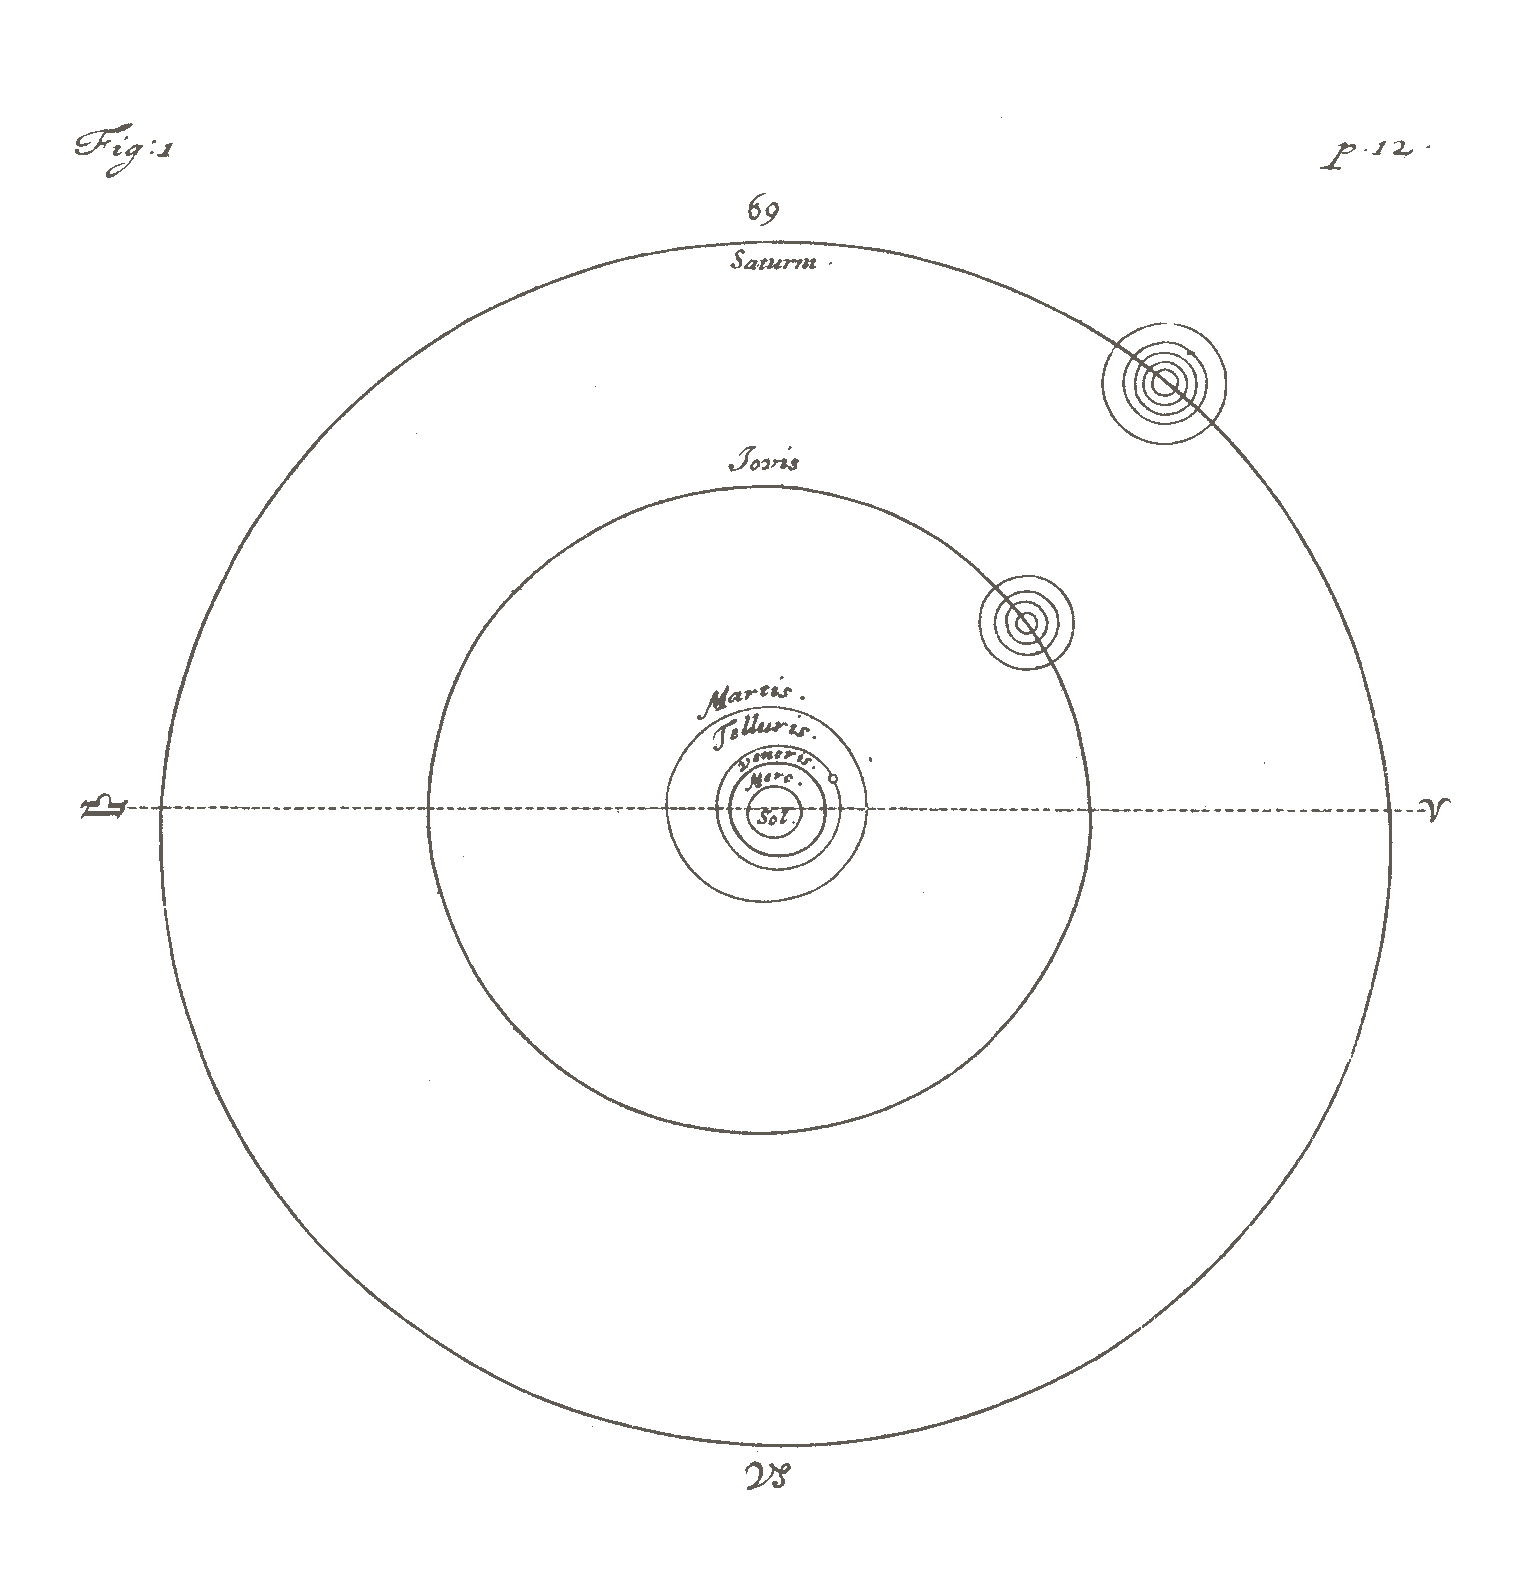
\includegraphics[width=.90 \textwidth]{ct_1_en.jpg}
\end{center}


The first is a Description of the Orbs the Planets move
in, in that order that they are placed round the Sun, drawn as near as can
be in their true Proportions, like what you have seen in my Clock at home.
The second shows the Proportions of their Magnitudes in respect of one
another and of the [12] Sun, which you know is upon that same Clock of mine
too. In the first the middle Point or Center is the Place of the Sun, round
which, in an order that everyone knows, are the Orbits of Mercury, Venus,
the Earth with that of the Moon about it; then those of Mars, Jupiter and
Saturn: and about the two last the small Circles that their Attendents march
in: about Jupiter four, and about Saturn five. Which Circles as well as that
of the Moon are drawn larger than their true Proportion would admit,
otherwise they could not have been seen. You may easily apprehend the
Vastness of these Orbits by this, that the distance of the Earth from the
Sun is ten or twelve thousand of the Earth's Diameters. Almost all these
Circles are in the same Plane, declining very little from that in which the
Earth moves, call'd the Plane of the Ecliptick. This Plane is cut obliquely
by the Axis upon which the Earth turns it self round in 24 hours, whence
arise the Successions of Day and Night: The Axis of the Earth always
keep[13]ing the same Inclination to the Ecliptick (except a small change
best known to Astronomers) while the Earth it self is carry'd in its yearly
Course round the Sun, causes the regular Order of the Seasons of the Year:
as you may see in all Astronomers Books.  Out of which I shall transcribe
hither the Periods of the Revolutions of the Planets, viz. Saturn moves
round the Sun in 29 Years, 174 Days, and 5 Hours: Jupiter finishes his
Course in 11 Years, 317 Days, and 15 Hours: Mars his in about 687 Days. Our
Year is 365 Days 6 Hours: Venus's 224 Days 18 Hours: and Mercury's 88 Days.
This is the now commonly receiv'd System, invented by Copernicus, and very
agreeable to that frugal Simplicity Nature shows in all her Works.


\section{Arguments for the truth of it}

If any one is resolved to find fault with it, let him first be sure he
understands it. Let him first see in the Books of Astronomers with how much
greater ease and plainness all the Motions of the Stars, and Appearances in
the Heavens are explained and demonstrated in this than either in [14] that
of Ptolemy or Tycho. Let him consider that Discovery of Kepler, that the
distances of the Planets from the Sun, as well of the Earth as the rest; are
in a fixt certain proportion to the times they spend in their Revolutions.
Which Proportion it's since observed that their Satellites keep round
Jupiter and Saturn. Let him examine what a contradictory Motion they are
fain to invent for the solution of the Polar Star's changing its distance
from the Pole. For that Star in the end of the Little Bear's Tail which now
describes so small a Circle round the Pole, that it is not above two Degrees
and twenty Minutes, was observed about 1820 Years ago, in the time of
Hipparchus, to be above 12: and will within a few ages more be forty five
Degrees distant from it: and after 25000 years more will return to the same
place it is now in. Now if with them we allow the Heavens to be turned upon
their own Axis, at this rate they must have a new Axis every day: a thing
most abominably absurd, and repugnant to the nature of all motion.
Where[15]as nothing is easier with Copernicus than to give us satisfaction
in this matter. Then he may impartially weigh those Answers that Galileus,
Gassendus, Kepler, and others have given to all Objections proposed, which
have so satisfied all Scruples, that generally all Astronomers now adays are
brought over to our side, and allow the Earth its Motion and Place among the
Planets. If he cannot be satisfied with all this, he is either one whose
Dulness can't comprehend it, or who has his Faith at another man's disposal,
and so for fear of Galileo's fate dare not own it.

\begin{center}
	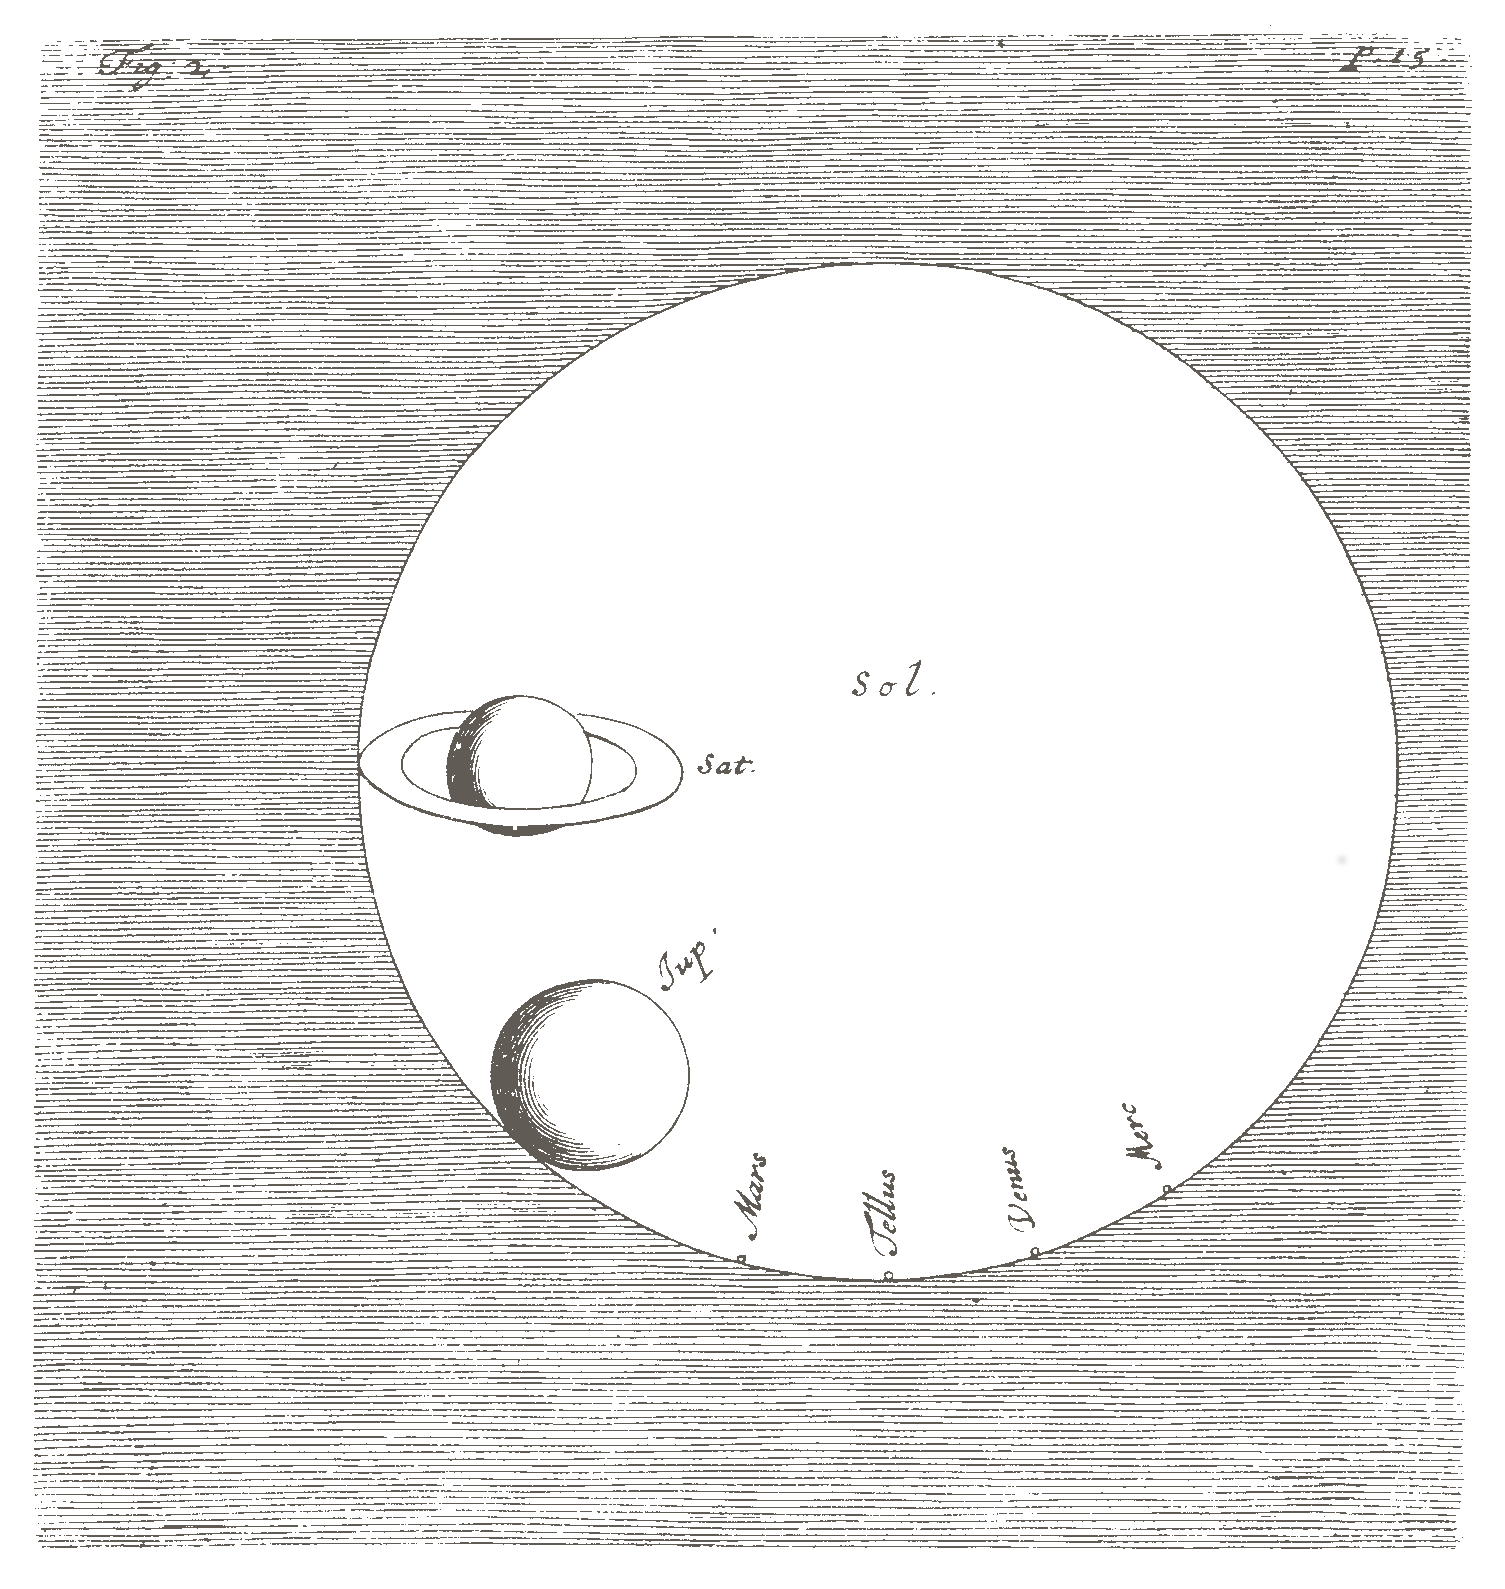
\includegraphics[width=.90 \textwidth]{ct_2_en.jpg}
\end{center}


\section{The Proportion of the Magnitude of the Planets, in
respect of one another, and the Sun}

In the other Figure you have the Globes of the Planets, and of the Sun,
represented to your eyes as plac'd near one another. Where I have observ'd
the same Proportion of their Diameters to that of the Sun, that I publish'd
to the World in my Book of the Appearances of Saturn: namely, the Diameter
of the Ring round Saturn is to that of the Sun as 11 is to 37; that of
Saturn himself about as 5 to 37; that of Jupiter as 2 to 11; that [16] of
Mars as 1 to 166; of the Earth as 1 to 111; and of Venus as 1 to 84: to
which I shall now add that of Mercury observ'd by Hevelius in the Year 1661,
but calculated by my self, and found to be as 1 to 290.


\section{The Lamellæ more convenient than Micrometers}

If you would know the way that we came to this knowledg of their Magni-
tudes, by knowing the Proportion of their Distances from the Sun, and the
measure of their Diameters, you may find it in the Book beforementioned:
and I cannot yet see any reason to make an alteration in those I then settled,
altho I will not say they are without their faults.
For I can't yet be of their mind, who think the use of micrometers, as
they call them, is beyond that of our Plates, but must still think that those
thin Plates or Rods of which I there taught the use, not to detract from
the due praises of so useful an Invention, are more convenient than the
Micrometers.


\section{The Earth justly liken'd to the Planets, and the
Planets to it}

In this Proportion of the Planets it is worth while to take notice of the
prodigious Magnitude of the Sun in comparison with the four innermost, [17]
which are far less than Jupiter and Saturn. And ‘tis remarkable, that the
Bodies of the Planets do not increase together with their distances from the
Sun, but that Venus is much bigger than Mars.  Having thus explain'd the two
Schemes, there's no body I suppose but, sees, that in the first the Earth is
made to be of the same sort with the rest of the Planets. For the very
Position of the Circles shows it. And that the other Planets are round like
it, and like it receive all the Light they have from the Sun, there's no
room (since the Discoveries made by Telescopes) to doubt, Another thing they
are like it in is, that they are moved round their own Axis; for since 'tis
certain that Jupiter and Saturn are, who can doubt it of the others? Again,
as the Earth has its Moon moving round it, so Jupiter and Saturn have
theirs. Now since in so many things they thus agree, what can be more
probable than that in others they agree too; and that the other Planets are
as beautiful and as well stock'd with [18] Inhabitants as the Earth? or what
shadow of Reason can there be why they should not?  If anyone should be at
the dissection of a Dog, and be: there shewn the Intrails, the Heart,
Stomach, Liver, Lungs and Guts, all the Veins, Arteries and Nerves; could
such a Man reasonably doubt whether there were the same Contexture and
Variety of Parts in a Bullock, Hog, or any other Beast, tho he had never
chanc'd to see the like opening of them? I don't believe he would. Or were
we thorowly satisfy'd in the Nature of one of the Moons round Jupiter,
should not we straight conclude the same of the rest of them?  So if we
could be assur'd in but one Comet, what it was that is the cause of that
strange appearance, should we not make that a Standard to judg of all others
by?


\section{Arguments from their Similitude of no small weight}

'Tis therefore an Argument of no small weight that is fetch'd from Relation
and Likeness; and to reason from what we see and are sure of, to what we
cannot, is no false Logick. This must be our Method in this Treatise, [19]
wherein from the Nature and Circumstances of that Planet which we see
before our eyes, we may guess at those that are farther distant from us.


\section{The Planets are solid, and not without Gravity}

And; First, 'tis more than probable that the Bodies of the Planets are solid
like that of our Earth, and that they don't want what we call Gravity, that
Virtue, which like a Loadstone attracts whatsoever is near the Body to its
Center. And that they have such a quality, their very Figure is a proof; for
their Roundness proceeds only from an equal pressure of all their Parts
tending to the same Center. Nay more, we are so skilful now adays, as to be
able to tell how much more or less the Gravitation in Jupiter or Saturn is
than here; of which Discovery and its Author you may read my Essay of the
Causes of Gravitation.


\section{Have Animals and Plants}

But now to carry the search farther, let us see by what steps we must rise
to the attaining some knowlege in the more private Secrets concerning the
State and Furniture of these new Earths. And, first, how likely is it [20]
that they may be stock'd with Plants and Animals as well as we? I suppose no
body will deny but that there's somewhat more of Contrivance, some- what
more of Miracle in the production and growth of Plants and Animals, than in
lifeless heaps of inanimate Bodies, be they never so much larger; as
Mountains, Rocks, or Seas are. For the finger of God, and the Wisdom of
Divine Providence, is in them much more clearly manifested than in the
other. One of Democritus's or Cartes's Scholars may venture perhaps to give
some tolerable Explication of the appearances in Heaven and Earth, allow him
but his Atoms and Motion; but when he comes to Plants and An- imals, he'll
find himself non-plus'd, and give you no likely account of their Production.
For every thing in them is so exactly adapted to some design, every part of
them so fitted to its proper life, that they manifest an Infinite Wisdom,
and exquisite Knowlege in the Laws of Nature and Geometry, as, to omit those
Wonders in Generation, we shall by and by show; and [21] make it an
absurdity even to think of their being thus haply jumbled to- gether by a
chance Motion of I don't know what little Particles. Now should we allow the
Planets nothing but vast Deserts, lifeless and inanimate Stocks and Stones,
and deprive them of all those Creatures that more plainly speak their Divine
Architect, we should sink them below the Earth in Beauty and Dignity; a
thing that no Reason will permit, as I said before.  Well then, now we have
gain'd the Point for them, and the Planets may be allow'd some Bodys capable
of moving themselves, not at all inferior to ours, (for why should they?)
and these are Animals. Now for fear of starving there poor Creatures, we
must have Plants you know. And so the other Point is gain'd. And as for
their Growth and Nourishment, 'tis no doubt the same with ours, seeing they
have the same Sun to warm and enliven them as ours have.


\section{Not to be imagin'd too unlike ours}

But perhaps some body may say, we conclude too fast. They will not deny
indeed but that there may be [22] Plants and Animals on the Surface of the
Planets, that deserve as well to be provided for by their Creator as ours
do: but why must they be of the same nature with ours? Nature seems to court
variety in her Works, and may have made them widely different from ours
either in their matter or manner of Growth, in their outward Shape, or their
inward Contexture; she may have made them such as neither our Understanding
nor Imagination can conceive. That's the thing we shall now examin, and
whether it be not more likely that she has not observ'd such a variety as
they talk of. Nature seems most commonly, and in most of her Works, to
affect Variety, 'tis true; But they should consider 'tis not the business of a
man to pretend to settle how great this Difference and Variety must be. Nor
does it follow, because it may be Infinite, and out of our comprehension and
reach, that therefore things in reality are so. For suppose God should have
pleased to have made all things there just as he has here, the Inhabitants
of those Places (if there [23] are any such strange things) would admire his
Wisdom and Contrivance no less than if they were widely different; seeing
they can't come to know what's done in the other Planets.  Who doubts but
that God, if he had pleased, might have made the Animals in America and
other distant Countries nothing like ours? (and Nature you know affects
Variety) yet we see he has not done it. They have indeed some difference in
their shape, and 'tis fit they should, to distinguish the Plants and Animals
of those Countries from ours, who live on this side the Earth; but even in
this variety there is an Agreement, an exact Correspondence in figure and
shape, the same ways of Growth, and new Productions, and of continuing their
own kind. Their Animals have Feet and Wings like ours, and like ours have
Heart, Lungs, Guts, and the Parts serving to Generation; whereas all these
things, as well with them as us, might, if it had so pleased Infinite
Wisdom, have been order'd a very different way. 'Tis plain then that
Na[24]ture has not exhibited that Variety in her Works that she could, and
therefore we must not allow that weight to this Argument, as upon the
account of it to make every thing in the Planets quite different from what
is here. 'Tis more probable that all the difference there is between us and
them, springs from the greater or less distance and influence from that
Fountain of Heat and Life the Sun; which will cause a difference not so much
in their Form and Shape, as in their Matter and Contexture.


\section{Planets have Water}

And as for the matter whereof the Plants and Animals there consist, tho it
is impossible ever to come to the knowlege of its Nature, yet this we may
venture to assert (there being scarce any doubt of it) that their Growth and
Nourishment proceeds from some liquid Principle. Far all Philosophers agree
that there can be no other way of Nutrition; some of the chief among them
having made Water to be the Original of all things: Far whatsoever's dry and
without moisture, is without motion too; and [25] without motion it's
impossible there should be any increase. But the parts of a Liquid being in
continual motion one with another, and insinuating and twisting them- selves
into the smallest Places, are thereby very proper and apt to add not
themselves only, but whatsoever else they may bring along with them to the
increase and growth of Bodies. Thus we see that by the means of Water the
Plants grow, blossom, and bear Fruit; and by the addition of that only,
Stones grow together out of Sand. And there's no doubt but that Metals,
Crystals, and Jewels, have the same method of Production: Tho in them there
has been no opportunity to make the same observation, as well by reason of
their slow advances, as that they are commonly found far from the Places of
their Generation; thrown up I suppose by some Earthquakes or Convulsions.
That the Planets are not without Water, is made not im- probable by the late
Observations: For about Jupiter are observ'd some spots of a darker hue than
the rest of his Body, [26] which by their continual change show themselves
to be Clouds: For the spots of Jupiter which belong to him, and never remove
from him, are quite different from these, being sometimes for a long time
not to be seen for these Clouds; and again, when there disappear, showing
themselves. And at the going off of these Clouds, some spots have been taken
notice of in him, much brighter than the rest of his Body, which remain'd
but a little while, and then were hid from our sight. These Monsieur Cassini
thinks are only the Reflection from the Snow that covers the tops of the
Hills in Jupiter: but I should rather think that it is only the colour of
the Earth, which chances to be free from those Clouds that commonly darken
it.  Mars too is found not to be without his dark spots, by means of which
he has been observ'd to turn round his own Axis in 24 hours and 40 minutes;
the length of his day: but whether he has Clouds or no, we have not had the
same opportunity of observing as in Jupiter, as well because even when [27]
he is nearest the Earth, he appears to us much less than Jupiter, as that
his Light not coming so long a Journey, is so brisk as to be an Impediment
to exact Observations: And this Reason is as much stronger in Venus as its
Light is. But since 'tis certain that the Earth and Jupiter have their Water
and Clouds, there is no reason why the other Planets should be without them.


\section{But not just like ours}

I can't say that they are exactly of the same nature with our Water; but
that they should be liquid their use requires, as their beauty does that they
should be clear. For this Water of ours, in Jupiter or Saturn, would be
frozen up instantly by reason of the vast distance of the Sun. Every Planet
therefore must have its Waters of such a temper, as to be proportion'd to
its heat: Jupiter's and Saturn's must be of such a nature as not to be liable
to Frost; and Venus's and Mercury's of such, as not to be easily evaporated
by the Sun. But in all of them, for a continual supply of Moisture, whatever
Water is drawn up by the Heat of the Sun into Vapors, must necessa[28]rily
return back again thither. And this it cannot do but in drops, which are
caused as well there as with us, by their ascending into a higher and colder
Region of the Air, out of that which, by reason of the Reflection of the Rays
of the Sun from the Earth, is warmer and more temperate.


\section{Plants grow and are nourish'd there as they are here}

Here then we have found in there new Worlds Fields warm'd by the kindly Heat
of the Sun, and water'd with fruitful Dews and Showers: That there must be
Plants in them as well for Ornament as Use, we have shewn just now. And what
Nourishment, what manner of Growth shall we allow them?  Why, I think there
can be no better, nay no other, than what we here experience; by having
their Roots fastned into the Earth, and imbibing its nourishing Juices by
their tender Fibres. And lest they should be only like so many bare Heaths,
with nothing but creeping Shrubs and Bushes, we'll e'en send them some
nobler and loftier Plants, Trees, or somewhat like them: These being the
greatest, and, except Waters, the only [29] Ornament that Nature has
bestow'd upon the Earth. For not to speak of those many uses that are made
of their Wood, there's no one that is ignorant either of their Beauty or
Pleasantness. Now what way can anyone imagine for a continual Production and
Succession of these Plants, but their bearing Seed? A Method so excellent
that it's the only one that Nature has here made use of, and so wonderful,
that it seems to be design'd not far this Earth alone. In fine, there's the
same reason to think that this Method is observ'd in those distant
Countries, as there was of its being follow'd in the remote Quarters of this
same Earth.


\section{The same true of their Animals}

'Tis much the same in Animals as 'tis in Plants, as to their manner of Nour-
ishment, and Propagation of their kind. For since all the living Creatures
of this Earth, whether Beasts, Birds, Fishes, Worms, or Insects, universally
and inviolably follow the same constant and fixt Institution of Nature; all
feed on Herbs, or Fruits, or the Flesh of other Animals that fed [30] on
them: since all Generation is perform'd by the impregnating of the Eggs, and
the Copulation of Male and Female: Why may not the same rule be observ'd in
the Planetary Worlds? For't is certain that the Herbs and Animals that are
there would be lost, their whole Species destroy'd without some daily new
Productions: except there be no such thing there as Misfortune or Ac-
cident: except the Plants are not like other humid Bodies, but can bear
Heat, Frost and Age, without being dry'd up, kill'd, or decay'd: except the
Animals have Bodies as hard and durable as Marble; which I think are gross
Absurdities. If we should invent some new way for their coming into the
World, and make them drop like Soland Geese from Trees, how ridiculous would
this be to any one that considers the vast difference between Wood and
Flesh? Or suppose we should have new ones made every day out of some such
fruitful Mud as that of Nile, who does not see how contrary this is to all
that's reasonable? And that 'tis much more agreeable to [31] the Wisdom of
God, once for all to create of all sorts of Animals, and distribute them all
over the Earth in such a wonderful and inconceivable way as he has, than to
be continually obliged to new Productions out of the Earth?  And what
miserable, what helpless Creatures must these be, when there's no one that
by his duty will be obliged, or by that strange natural fondness, which God
has wisely made a necessary argument for all Animals to take care of their
own, will be moved to assist, nurse or educate them?  As for what I have
said concerning their Propagation, I cannot be so positive; but the other
thing, namely, that they have Plants and Animals, I think I have fully
proved. And by the same Argument, of their not being inferiour to our Earth,
they must have as great a variety of both as we have. What this is, will be
best known to him that considers the different ways our Animals make use of
in moving from one place to another. Which may be reduc'd, I think, to
these; ei[32]ther that they walk upon two feet or four; or like Insects,
upon six, nay sometimes hundreds; or that they fly in the Air bearing up,
and wonderfully steering themselves with their Wings; or creep upon the
Ground without feet; or by a violent Spring in their Bodies, or paddling
with their feet, cut themselves a way in the Waters.  I don't believe, nor
can I conceive, that there should be any other way than these mention'd. The
Animals then in the Planets must make use of one or more of these, like our
amphibious Birds, which can swim in Water as well as walk on Land, or fly in
the Air; or like our Crocodiles and Sea-Horses, must be Mongrels, between
Land and Water. There can no other method be imagin'd but one of these. For
where is it possible for Animals to live, except upon such a solid Body as
our Earth, or a fluid one like the Water, or srill a more fluid one than
that, such as our Air is? The Air I confess may be much thicker and heavier
than ours, and so, without any disadvantage to its Transpa[33]rency, be
fitter for the volatile Animals. There may be too many sorts of Fluids
ranged over one another in rows as it were. The Sea perhaps may have such a
fluid lying on it, which tho ten times lighter than Water, may be a hundred
times heavier than Air; whose utmost Extent may not be so large as to cover
the higher places of their Earth. But there's no reason to suspect or allow
them this, since we have no such thing; and if we did, it would be of no
advantage to them, for that the former ways of moving would not be hereby at
all increas'd: But when we come to meddle with the Shape of these Creatures,
and consider the incredible variety that is even in those of the different
parts of this Earth, and that America has some which are no where else to be
found, I must then confess that I think it beyond the force of Imagination
to arrive at any knowlege in the matter, or reach probability concerning the
figures of these Planetary Animals. Altho considering these ways of Motion
we e'en now recounted; [34] they may perhaps be no more different from ours
than ours (those of ours I mean that are most unlike) are from one another.


\section{Great variety of Animals in this Earth}

If a man were admitted to a Survey of Jupiter or Venus, he would no doubt
find as great a number and variety as he had at home. Let us then, that we
may make as near a guess at, and as reasonable a judgment of the matter
as we can, consider the many sorts, and the admirable difference in the
shapes of our own Animals; running over some of the chief of them (for
'twould be tedious to set about a general Catalogue) that are notoriously
different from one another, either in their Figure or some peculiar Property
belonging to them; as they belong to the Land, or the Water, or the Air.
Among the Beasts we may take notice of the great distance between the
Horse, the Elephant, the Lion, the Stag, the Camel, the Hog, the Ape, the
Porcupine, the Tortoise, the Cameleon: in the Water, of that between the
Whale, and the Sea-Calf, the Skait, the Pike, the Eel, the Ink-[35]Fish, the
Pourcontrel, the Crocodile, the flying Fish, the Cramp Fish, the Crab, the
Oister, and the Purple Fish: and among Birds, of that between the Eagle,
the Ostrich, the Peacock, the Swan, the Owl, and the Bat: and in Insects,
of that between the Ants, the Spider, the Fly, and the Butterfly; and of that
Prodigy in their wonderful change from Worms. In this Roll I have pass'd
by the creeping kind as one sort, and skip'd over that vast multitude of less
different Animals that fill the intermediate spaces.


\section{And no less in the Planets}

But be they never so many, there is no reason to think that the Planets can-
not match them. For tho we in vain guess at the Figures of those Creatures,
yet we have discover'd somewhat of their manner of Life in general; and of
their Senses we shall more by and by.


\section{Rational Animals in the Planets}

But still the main and most diverting Point of the Enquiry is behind, which
is the placing some Spectators in these new Discoveries, to enjoy these
Crea- tures we have planted them with, and to admire their Beauty and
Variety.  And among all, that have never so slightly meddled with these
matters, I don't find any that have scrupled to allow them their
Inhabitants: not Men perhaps like ours, but [37] some Creatures or other
endued with Reason.  For all this Furniture and Beauty the Planets are
stock'd with seem to have been made in vain, without any design or end,
unless there were some in them that might at the same time enjoy the Fruits,
and adore the wise Creator of them. But this alone would be no prevailing
Argument with me to allow them such Creatures. For what if we should say,
that God made them for no other design, but that he himself might see (not
as we do 'tis true; but that he that made the Eye sees, who can doubt?) and
delight himself in the contemplation of them? For was not Man himself, and
all that the whole World contains, made upon this very account? That which
makes me of this opinion, that those Worlds are not without such a Crea-
ture endued with Reason, is, that otherwise our Earth would have too much
the advantage of them, in being the only part of the Universe that could
boast of such a Creature so far above, not only Plants and Trees, but all
[38] Animals whatsoever: a Creature that has a Divine somewhat within him,
that knows, and understands, and remembers such an innumerable number of
things; that deliberates, weighs and judges of the Truth: a Creature upon
whose account, and for whose use, whatsoever the Earth brings forth seems to
be provided. For every thing here he converts to his own ends. With the
Trees, Stones, and Metals, he builds himself Houses: the Birds and Fishes he
sustains himself with: and the Water and Winds he makes subservient to his
Navigation; as he doth the sweet Smell and glorious Colours of the Flowers
to his Delight. What can there be in the Planets that can make up for its
Defects in the want of so noble an Animal? If we should allow Jupiter a
greater variety of other Creatures, more Trees, Herbs and Metals, all these
would not advantage or dignify that Planet so much as that one Animal doth
ours by the admirable Productions of his penetrating Wit. If I am out in
this, I do not know when [39] to trust my Reason, and must allow my self to
be but a poor Judg in the true estimate of things.


\section{Vices of Men no hindrance to their being the Glory of the Planet
they inhabit}

Nor let anyone say here, that there's so much Villany and Wickedness in this
Man that we have thus magnified, that it's a reasonable doubt, whether he
would not be so far from being the Glory and Ornament of the Planet that
enjoys his Company, that he would be rather its Shame and Disgrace.  For
first, the Vices that most Men are tainted with, are no hindrance, but that
those that follow the Dictates of true Reason, and obey the Rules of a rigid
Virtue, are still a Beauty and Ornament to the place that has the happiness
to harbour them. Besides, the Vices of Men themselves are of excellent use,
and are not permitted and allow'd in the World without wise design. For
since it has so pleased God to order the Earth, and every thing in it as we
see it is (for it's nonsense to say it happen'd against his Will or
Knowlege) we must not think that those different Opinions, and that various
multiplicity of Minds [40] were plac'd in different Men to no end or
purpose: but that this mixture of bad Men with good, and the Consequents of
such a mixture, as Misfortunes, Wars, Afflictions, Poverty, and the like,
were given us for this very good end, viz. the exercising our Wits, and
sharpening our Inventions; by forcing us to provide for our own necessary
defence against our Enemies.  'Tis to the fear of Poverty and Misery that we
are beholden for all our Arts, and for that natural Knowlege which was the
product of laborious Industry; and which makes us that we cannot but admire
the Power and Wisdom of the Creator, which otherwise we might have pass'd by
with the same indifference as Beasts. And if Men were to lead their whole
Lives in an undisturb'd continual Peace, in no fear of Poverty, no danger of
War, I don't doubt they would live little better than Brutes, without all
knowlege or enjoyment of those Advantages that make our Lives pass on with
pleasure and profit. We should want the wonderful Art of Writing, if its
great [41] use and necessity in Commerce and War had not forc'd out the
Invention.  'Tis to these we owe our Art of Sailing, our Art of Sowing, and
most of those Discoveries of which we are Masters; and almost all the
Secrets in experi- mental Knowlege. So that those very things that make up
their Indictment against Reason, are no small helps to its advancement and
perfection. For those Virtues themselves, Fortitude and Constancy; would be
of no use if there were no Dangers, no Adversity, no Afflictions for their
exercise and trial.  If we should therefore imagine in the Planets some such
reasonable An- imal as Man is, adorn'd with the same Virtues, and infected
with the same Vices, it would be so far from degrading or vilifying them,
that while they want such a one, I must think them inferior to our Earth.


\section{Reason there not different from what 'tis here}

Well, but allowing these Planetarians some sort of Reason must it needs
be the same with ours? Why truly I think 'tis, and must be so; whether
we consider it as applied to Justice and [42] Morality, or exercised in the
Principles and Foundations of Science. For Reason with us is that which
gives us a true sense of Justice and Honesty, Praise, Kindness and Gratitude:
'tis that that teaches us to distinguish universally between Good and Bad;
and renders us capable of Knowlege and Experience in it. And can there be
any where a Reason contrary to this? or can what we call just and generous
in Jupiter or Mars be thought unjust Villany? This is not at all, I don't say
probable, but possible. For the aim and design of the Creator is every where
the preservation and safety of his Creatures. Now when such a Reason as
we are masters of, is necessary for the preservation of Life, and promoting
of Society (a thing that they be not without, as we shall show) would it not
be strange that the Planetarians should have such a perverse sort of Reason
given them, as would necessarily destroy and confound what it was design'd
to maintain and defend? But allowing Morality and Passions with those
Gentlemen to be somewhat [43] different from ours, and supposing they may
act by other principles in what belongs to Friendship, and Anger, Hatred,
Honesty, Modesty, and Comeliness, yet still there would be no doubt, but
that in the search after Truth, in judging of the Consequences of things, in
reasoning, particularly in that sort which belongs to Magnitude or Quantity,
about which their Geometry (if they have such a thing) is employ'd, there
would be no doubt I say, but that their Reason here must be exactly the
same, and go the same way to work with ours, and that what's true in one
part will hold true over the whole Universe; so that all the difference must
lie in the degrees of Knowlege, which will be proportional to the Genius and
Capacity of the Inhabitants.


\section{They have Senses}

But I perceive I am got a little too far: For till I have furnished them with
Senses, neither will Life be any pleasure to them, nor Reason of any use.
And I think it very probable, that all their Animals, as well their Beasts as
rational Creatures, are like [44] ours in all that relates to the Senses: For
without the power of Seeing we should find it impossible for Animals to
provide Food for themselves, or be forewarn'd of any approaching danger,
so as to guard themselves from it. So that where-ever we plant any Animals,
except we would have them lead the Life of Worms or Moles, we must allow
them Sight; than which nothing can conduce more either to the preservation
or pleasure of their Lives.


\section{Sight}

Then if we consider the wonderful nature of Light, and the amazing Artifice
in the fit framing the eye for the reception of it, we cannot but see that
Bodies so vastly remote could not be view'd by us in their proper Figures
and just Distances, any other way than by Sight. For this Sense, and all
others that we know of, must proceed from an external Motion. Which in the
sense of Seeing must come either from the Sun, the fixt Stars, or Fire:
whose Particles being whirled about with a rapid Motion, communicate it to
the Celestial Matter about, whence 'tis convey'd in an instant to the most
[45] distant parts, just like Sound through the Air. If it were not for this
Motion of the intermediate Matter, we should be all in darkness, and have
sight neither of Sun nor Stars, nor any thing else, for all other Light must
come to us at second-hand from them. This Motion perceived by the Eyes is
called Light. And the nice Curiosity of this Perception is admirable, in
that it is caused by the smallest Particle of that fine Matter, and can at
the same time determine the Coast from whence the Motion comes; in that all
these different Roads of Motion, these Waves crossing and interfering with
one another, are yet no hindrance to every ones free passage. All these
things are so wisely, so wonderfully contrived, that it's above the power of
humane Wit, not to invent or frame somewhat like them, but even to imagine
and comprehend them. For what can be more amazing, than that a Particle of
Body should be so devised and framed, as by its means to show us the Shape,
the Position, the Distance, and all the Motions, nay and all the [46]
Colours, distinguishing of a Body that is far remote from us? And then the
artful Composition of the Eye, drawing an exact Picture of the Objects
without it, upon the concave side of the Choroides, is even above all
admiration, nor is there any thing in which God has more plainly manifested
his excellent Geometry. And these things are not only contrived and framed
with so great Wisdom and Skill, as not to admit of better, but to any one
that considers them attentively, they seem to be of such a nature as not to
allow any other Method. For it's impossible that Light should represent
Objects to us at so vast a distance, except by such an intervening Motion;
and it's as impossible that any other Composition of the Eye should be
equally fitted to the reception of such Impressions. So that I cannot but
think them mightily out, that maintain these things might have been
contrived many other ways.  It's likely then, and credible, that in these
things the Planets have an exact correspondence with us, and that their
Animals [47] have the same Organs, and use the same way of sight that we do.
Well then they have Eyes, and two at least we must grant them, otherwise
they would not perceive some things close to them, and so could not avoid
Mischiefs that take them on the blind side. And if we must allow them all
Animals for the preservation of their Life, how much more must they that
make more, and more noble uses of them, not be deprived of the Blessing of
so advantageous Members? For by them we view the various Flowers, and the
elegant Features of Beauty: with them we read, we write, we contemplate the
Heavens and Stars, and measure their Distances, Magnitudes, and Journeys:
which how far they are common to the Inhabitants of those Worlds with us, I
shall strait examine.


\section{Hearing}

But first I shall enquire whether now we have given them one, we may not
venture upon the other four Senses, to make them as good Men as our selves.
And truly Hearing puts in hard, and almost perswades me to give it a share
in the Animals of those new Coun[48]tries. And 'tis of great consequence in
defending us from sudden accidents; and, especially when Seeing is of no use
to us, it supplys its place, and gives us seasonable warning of any imminent
danger. Besides, we see many Animals call their fellows to them with their
Voice, which Language may have more in it than we are aware of, tho we
don't understand it. But if we do but consider the vast uses and necessary
occasions of Speaking on the one side, and Hearing on the other, among
those Creatures that make use of their Reason, it will scarce seem credible
that two such useful, such excellent things were designed only for us. For
how is it possible but that they that are without these, must be without
many other Necessaries and Conveniences of Life? Or what can they have
to recompense this want?


\section{A Medium to convey Sound to the Ears}

Then, if we go still farther, and do but meditate upon the neat and frugal
Contrivance of Nature in making this same Air, by the drawing in of which we
live, by whose Motion we sail, and by whose means Birds fly, for a [49]
conveyance of Sound to our ears; and this Sound for the conveyance of
another man's Thoughts to our Minds: can we ever imagin that she has left
those other Worlds destitute of so vast Advantages? That they don't want the
means of them is certain, for their having Clouds in Jupiter puts it past
doubt that they have Air too; that being mostly formed of the Particles of
Water flying about, as the Clouds are of them gathered into small Drops.
And another proof of it is, the necessity of breathing for the preservation
of Life, a thing that seems to be as universal a Dictate of Nature, as
feeding upon the Fruits of the Earth.


\section{Touch}

As for Feeling, it seems to be given upon necessity to all Creatures that
are cover'd with a fine and sensible Skin, as a Caution against coming too
near those things that may injure or incommode them: and without it they
would be liable to continual Wounds, Blows and Bruises. Nature seems to have
been so sensible of this; that she has not left the least place free from
such a perception. Therefore it's pro[50]bable that the Inhabitants of those
Worlds are not without so necessary a Defence, and so fit a Preservative
against Dangers and Mishaps.


\section{Smell and Tast}

And who is there that doth not see the inevitable necessity for all Creatures
that live by feeding to have both Tast and Smell, that they may distinguish
those things that are good and nourishing, from those that are mischievous
and harmful? If therefore we allow the Planetary Creatures to feed upon
Herbs, Seeds, or Flesh, we must allow them a distinguishing Tast and Smell
too, that they may chuse or refuse any thing according as they find it likely
to be advantagious or noxious to them.


\section{Their Senses not very different from ours}

I know that it hath been a question with many, whether there might not
have been more Senses than those five. If we should allow this, it might
nevertheless be reasonably doubted whether the Senses of the Planetary
Inhabitants are much different from ours. I must confess, I cannot deny but
there might possibly have been more Senses; but when I consider the Uses
[51] of those we have, I cannot think but they would have been superfluous.
The Eye was made to discern near and remote Objects, the Ear to give us
notice of what our Eyes could not, either in the dark or behind our back:
Then what neither the Eye nor the Ear could, the Nose was made (which in
Dogs is wonderfully nice) to warn us of. And what escapes the notice of the
other four Senses, we have Feeling to inform us of the too near approaches
of, before it can do us any mischief. Thus has Nature so plentifully, so
perfectly provided for the necessary preservation of her Creatures here, that
I think she can give nothing more to those there, but what will be needless
and superfluous. Yet the Senses were not wholly design'd for use: but Men
from all, and all other Animals from some of them, reap Pleasure as well
as Profit, as from the Tast in delicious Meats; from the Smell in Flowers
and Perfumes; from the Sight in the contemplation of beauteous Shapes
and Colours; from the Hearing in the sweetness and har[52]mony of Sounds;
from the Feeling in Venery, unless you please to count that for a particular
Sense by it self.


\section{They have Pleasure arising from the Senses}

Since it is thus, I think 'tis but reasonable to allow the Inhabitants of
the Planets these same advantages that we have from them. For upon this con-
sideration only, how much happier and easier a man's Life is render'd by the
enjoyment of them, we must be obliged to grant them these Blessings, except
we would ingross every thing that is good to our selves, as if we were
worthier and more deserving than any else. But moreover, that Pleasure which
we perceive in eating or in copulation, seems to be a necessary and
provident Command of Nature, whereby it tacitly compels us to the preser-
vation and continuance of our Life and Kind. It is the same in Beasts. So
that both for their happiness and preservation it's very probable the rest
of the Planets are not without it. Certainly when I consider all these
things, how great, noble, and useful they are; when I consider what an
admirable Providence it is [53] that there's such a thing as Pleasure in the
World, I can't but think that our Earth, the smallest part almost of the
Universe, was never design'd to monopolize so great a Blessing. And thus
much for those Pleasures which affect our bodily Senses, but have little or
no relation to our Reason and Mind. But there are other Pleasures which Men
enjoy, which their Soul only and Reason can relish: some airy and brisk,
others grave and solid, and yet nevertheless Pleasures, as arising from the
Satisfac- tion which we feel in Knowlege and Inventions, and searches after
Truth, of which whether the Planetary Inhabitants are not partakers, we
shall have an opportunity of enquiring by and by.  There are some other
things to be consider'd first, in which it's probable they have some
relation to us. That the Planets have those Elements of Earth, Air, and
Water, as well as we, I have already made not unlikely.


\section{All the Planets have Fire}

Let us now see whether they may not have Fire too: which is not so properly
call'd an Element, as a rapid [54] Motion of the Particles in the
inflammable Body. But be it what it will, there are many Arguments for their
not being without it. For this Earth is not so truly call'd the Place of
Fire as the Sun: and as by the heat of that all Plants and Animals here
thrive and live; so, no doubt, is it in the other Planets. Since then Fire
is caused by a most intense and vigorous Heat, it follows that the Planets,
especially those nearer the Fountain of it, have their proportionate degrees
of Heat and Fire. And when there are so many ways of its Production, as by
the collection of the Rays of the Sun, by the reflection of Mirrors, by the
striking of Flint and Steel, by the rubbing of Wood, by the close loading of
moist Grass, by Lightning, by the eruptions of Mountains and Volcanos, it's
strange if neither Art should have produc'd it, nor Nature effected it there
by one of these many means.  Then how useful and necessary is it to us? By
it we drive away Cold, and supply the want of the Sun in those Countries
where his oblique Rays [55] make a less vigorous Impression, and so keep a
great part of the Earth from being an uninhabited Desart: which is equally
necessary in all the Planets, whether we allow them Succession of Seasons,
or a, perpetual Spring and Æquinox: for even then the Countries near the
Pole would receive but little advantage from the Heat of the Sun. By the
help of this we turn the night into day, and thereby make a considerable
addition to the shortness so our Lives. Upon all these accounts I must not
let this Earth of ours enjoy it all alone, and exclude all the other Planets
from so advantageous and so profitable a Gift.


\section{The bigness of their Creatures not rightly guest at by the bigness
of the Planets}

But perhaps it maybe asked as well concerning Brutes as rational Creatures,
and of their Plants and Trees too, whether they are proportionably larger or
less than ours. For if the Magnitude of the Planets was to be the Standard
of their measure, there would be Animals in Jupiter ten or fifteen times
larger than Elephants, and as much longer than our Whales. And then their
Men must be mere Goliahs, [56] in respect of our Pygmiships. Now tho I don't
see any so great absurdity in this as to make it impossible, yet there is no
reason to think it is really so, seeing Nature has not always ty'd her self
to those Rules which we have thought more convenient for her: for example,
the magnitude of the Planets is not answerable to their distances from the
Sun; but Mars, tho more remote, is far less than Venus: and Jupiter turns
round his Axis in ten hours, when the Earth which is much lees than him,
spends 24. But since Nature, perhaps some body will say, has not observ'd
such a Regularity in the proportion of things, for ought we know we may have a
Race of Pygmies about the bigness of Frogs and Mice, possess'd of the
Planets. But I shall show that this is very improbable by and by.


\section{In the Planets are many sorts of rational Creatures as well as here}

There may arise another Question, whether there be in the Planets but one or
more sorts of rational Creatures possess'd of different degrees of Reason
and Sense. There is something not unlike this to be observ'd among [57] us.
For to pass by those who have human Shape (altho some of them would very
well bear that enquiry too) if we do but consider some sorts of Beasts, as
the Dog, the Ape, the Beaver, the Elephant, nay some Birds and Bees, what
sense and Understanding they are masters of, we shall be forc'd to allow,
that Man is not the only rational Animal. For we discover somewhat in them
of Reason independent on, and prior to all teaching and practice.  But still
no body can doubt, but that the Understanding and Reason of Man is to be
prefer'd to theirs as being comprehensive of innumerable things, indued with
an infinite memory of what's past, and capable of providing against what's
to come. That there is some such rational Creature in the other Planets,
which is the Head and Sovereign of the rest, is very reasonable to believe:
for otherwise, were many endued with the same Wisdom and Cunning, we should
have them always doing mischief, always quarrelling and fighting one another
[58] for Empire and Sovereignty, a thing that we feel too much of where we
have but one such Creature. But to let that pass, our next Enquiry shall be
concerning those Animals in the Planets which are furnish'd with the
greatest Reason, whether it's possible to know wherein they employ it, and
whether they have made as great advances in Arts and Knowlege as we in our
Planet. Which deserves most to be consider'd and examin'd of any thing
belonging to their nature; and for the better performance of it we must take
our rise somewhat higher, and nicely view the Lives and Studies of Men.  And
in those things wherein Men provide and take care only of what's ah-
solutely necessary for the preservation of their Life; in defending
themselves from the Injuries of the Air; in securing themselves against the
Incursions of Enemies by Walls; and against Fraud and Disturbances by Laws;
in edu- cating their Children, and providing for themselves and them: In all
these I can see no great [59] reason that Man has to boast of the
preeminency of his Reason above Beasts and other Animals. For most of these
things they per- form with greater ease and art than us, and some of them
they have no need of. For that sense of Virtue and Justice in which Man
excels, of Friendship, Gratitude and Honesty, of what use are they, but
either to put a stop to the Wickedness of Men, or to secure us from mutual
Assaults and Injuries, a thing wherein the Beasts want no Guide but Nature
and Inclination? Then if we set before our eyes the manifold Cares, the
disturbances of Mind, the restless Desires, the dread of Death, that are the
result of this our Reason; and compare them with that easy, quiet, and
harmless Life which other An- imals enjoy, we should be apt to wish a
change, and conclude that they, especially Birds, liv'd with more pleasure
and happiness than Man could with all his Wisdom. For they have as great a
gusto of bodily Pleasures as we, let the new Philosophers say what they
will, who would [60] have them go for nothing but Clocks and Engines of
Flesh; a thing which Beasts so plainly confute by crying and running away
from a stick, and all other actions, that I wonder how anyone could
subscribe to so absurd and cruel an Opinion. Nay I can scarce doubt but that
Birds feel no small pleasure in their easy, smooth sailing through the Air;
and would much more if they but knew the advantages it hath above our slow
and laborious Progression.



\section{Men chiefly differ from Beasts in the study of Nature}

What is it then after all that sets human Reason above all other, and makes
us preferable to the rest of the Animal World? Nothing in my mind so much
as the contemplation of the Works of God, and the study of Nature, and
the improving those Sciences which may bring us to some knowlege in their
Beauty and Variety. For without Knowlege what would be Contemplation?
And what difference is there between a Man, who with a careless supine neg-
ligence views the Beauty and Use of the Sun, and the fine golden Furniture
of the Heaven, and one [61] who with a learned Niceness searches into their
Courses; who understands wherein the Fixt Stars, as they are call'd, differ
from the Planets, and what is the reason of the regular Vicissitude of the
Seasons; who by sound reasoning can measure the magnitude and distance
of the Sun and Planets? Or between such a one as admires perhaps the
nimble Activity and strange Motions of some Animals, and one that knows
their whole Structure, understands the whole Fabrick and Architecture of
their Composition?


\section{They have Astronomy}

If therefore the Principle we before laid down be true, that the other
Planets are not inferior in dignity to ours, what follows but that they have
Creatures not to stare and wonder at the Works of Nature only, but who
employ their Reason in the examination and knowlege of them, and have made
as great advances therein as we have? They do not only view the Stars, but
they improve the Science of Astronomy: nor is there any thing can make us
think this improbable, but that fond conceitedness of every thing that we
[62] call our own, and that pride that is too natural to us to be easily
laid down. But I know some will say, we are a little too bold in these
Assertions of the Planets, and that we mounted hither by many Probabilities,
one of which, if it chance to be false, and contrary to our supposition,
would, like a bad Foundation, ruin the whole Building, and make it fall to
the ground.  But I would have them to know, that all I have said of their
Knowlege in Astronomy, has proofs enough, antecedent to those we now
produc'd. For supposing the Earth, as we did, one of the Planets of equal
dignity and honor with the rest, who would Venture to say, that no where
else were to be found any that enjoy'd the glorious sight of Nature's Opera?
Or if there were any fellow-Spectators, yet we were the only ones that had
dived deep into the secrets and knowlege of it? So then here's a proof not
so far fetch'd for the Astronomy of the Planets, the same which we used for
their having rational Creatures, and enjoying the other advan[63]tages we
before talk'd of, which serves at the same time for the confirmation of our
former Conjectures. But if Amazement and Fear at the Eclipses of the Moon
and Sun gave the first occasion to the study of Astronomy, as they say it
did, then it's almost impossible that Jupiter and Saturn should be without
it; the Argument being of much greater force in them, by reason of the;
daily Eclipses of their Moons, and the frequent ones of the Sun to their
Inhabitants. So that if a Person disinterested in his Judgment, and equally
ignorant of the Affairs of all the Planets, were to give his Opinion in the
matter, I don't doubt he would give the cause for Astronomy to those two
Planets rather than us.  This supposition of their Knowlege and Use of
Astronomy in the Plane- tary World, will afford us many new Conjectures
about their manner of life, and their state as to other things.


\section{And all its subservient Arts}

For, First: No Observations of the Stars, that are necessary to the knowlege
of their Motions, can be made without Instruments; nor can [64] these be
made without Metal, Wood, or some such solid Body. Here's a necessity of
allowing them the Carpenters Tools, the Saw, the Ax, the Plane, the Mallet,
the File: and the making of these requires the use of Iron, or some equally
hard Metal.


\section{Geometry and Arithmetick}

Again, these Instruments can't be without a Circle divided into equal Parts,
or a streight line into unequal. Here's a necessity for introducing Geometry
and Arithmetick.



\section{And Writing}

Then the necessity in such Observations of marking down the Epochas or
Accounts of Time, and of transmitting them to Posterity, will force us to
grant them the Art of Writing; I won't say the same with ours which is
commonly used, but I dare affirm not more ingenious or easy. For how
much more ready and expeditious is our way, than by that multitude of
Characters used in China; and how vastly preferable to Knots tied in Cords,
or the Pictures in use; among the barbarous People of Mexico and Peru?
There's no Nation in the World but has some way or other of writing and
marking down [65] their Thoughts: So that it's no wonder if the Planetarians
have been taught it by that great School-mistress Necessity, and apply it to
the study of Astronomy and other Sciences. In Astronomical matters the
necessity of it is moreover apparent from hence, that the motion of the
Stars is as 'twere to be fancied and guess'd at in different Systems, and
these Systems to be continually improved and corrected, as later and more
exact Observations shall convince the old ones of faults: all which can never
be deliver'd down to succeeding Generations, unless we make use of Letters
and Figures.


\section{And Opticks}

But for all our large and liberal allowances to these Gentlemen, they will
still be behind-hand with us, For we have so certain a knowlege of the
true System and Frame of the Universe; we have so admirable an Invention
of Telescopes to help our failing Eye-sight in the view of the bigness and
different forms of the Planetary Bodies, in the discovery of the Mountains,
and the Shadows of them on [66] the Surface of the Moon, in the bringing
to light an innumerable multitude of Stars otherwise invisible, that we must
necessarily be far their Masters in that Knowlege. What must I do here? I
could find in my heart (and I can see no reason why I may not, except it
be to flatter and complement our selves in being the only People that have
the advantage of such excellent Inventions) either to allow these Planetary
Inhabitants such sharp Eyes as not to need them, or else the use of Glasses
to help the deficiency of their Sight. And yet I dare not, for fear People
should be so disturbed at the ridiculous Extravagancy of such an Opinion,
as to take the measure of my other Conjectures by it, and hiss them all off,
upon the account of this alone.


\section{These Sciences not contrary to Nature}

But some body may perhaps object, and that not without reason at first
sight, that the Planetarians it's likely are destitute of all refined
Knowlege, just as the Americans were before they had Commerce with the
Europeans.  For if one considers the Ignorance of [67] those Nations, and of
others in Asia and Africa equally barbarous, it will appear as if the main
design of the Creator in placing Men upon the Earth was that they might
live, and, in a just sense of all the Blessings and Pleasure they enjoy,
worship the Fountain of their Happiness; but that some bold fellows have
leapt over the bounds of Nature, and made searches into those forbidden
depths only out of an affectation of knowing more than they were made for.
There does not want an Answer for these Men. For God could not but foresee
the advances Men would make, in their enquiring into the Affairs of Heaven:
that they would discover Arts useful and advantageous to Life: that they
would cross the Seas, and dig up the Bowels of the Earth. Nothing of all
this could happen contrary to the Mind and Knowlege of the Infinite Author
of all things. And if he foresaw these things would be, he so appointed and
destin'd them to human kind. And the Studies of Arts and Sciences cannot be
said to be con[68]trary to Nature, since in the search thereof they are
employ'd: especially if we consider the natural desire and love of Knowlege,
rooted in all men. For it's impossible this should have been given them upon
no design or account. But they will urge, that if such a Knowlege is
natural, if we were born for it, why are there so very few, especially in
Astronomy, that prosecute these Studies? For Europe is the only Quarter of
the Earth in which there have been any advancements made in Astronomy. And
as for the Judicial Astrology, that pretends to foretel what is to come, it
is such a ridiculous, and oftentimes mischievous Folly, that I do not think
it fit to be so much as named. And even in Europe, not one in a hundred
thousand meddles with these Studies. Besides, its Original and Rise is so
late, that many Ages were past before the very first Rudiments of Astronomy
or Geometry (which is necessary to the learning of it) were known. For every
body is acquainted almost with its first beginnings in Egypt and Greece.
Add to [69] this, that 'tis not yet above fourscore years since the bungling
Epicycles were discarded, and the true and easy plain Motion of the Planets
was discover'd. For the satisfaction of these Scruples, to what we said
before, concerning the Fore-knowlege of God, may be added this; That God
never design'd we should come into the World Astronomers or Philosophers ;
these Arts are not infus'd into us at our birth, but were order'd, in long
tracts of Time, by degrees to be the rewards and result of laborious
Diligence: especially those Sciences which are now in debate, are so much
the more difficult and abstruse, that their late Invention and slow Progress
are so far from being a wonder, that it is rather strange they were ever
discover'd at all. There are but few, I acknowlege one or two perhaps, in an
age, that pursue them, or think them their business: but their number will
be very considerable if we take in those that have liv'd in all the ages in
which Astronomy hath flourished: and no body can deny them that happiness
and contentment which [70] they have pretended to above all others. In fine,
it was sufficient that so small a number should make it their study; so that
the Profit and Advantage of their Inventions might but spread it self over
all the World. Since then the Inhabitants of this Earth, let them be never
so few, have had Parts and Genius sufficient for the attainment of this
Knowlege; and there's no reason to think the Planetarians less ingenious or
happy than our selves; we have gained our point, and 'tis probable that they
are as skilful Astronomers as we can pretend to be. So that now we may
venture to deduce some Consequences from such a Supposition.  We have before
show'd the necessary Dependence and Connexion, not only of Geometry and
Arithmetick, but of mechanical Arts and Instruments with this Science. This
leads us naturally to the enquiry how they can use these Instruments and
Engines for the observation of the Stars, how they can write down such their
Observations, and perform other things which we do with our hands.


\section{They have Hands}

So [71] that we must necessarily give them hands, or some other Member, as
convenient for all those uses, instead of them. I know an antient
Philosopher laid such stress upon the use and conveniency of the hands, that
he made no scruple to affirm, they were the cause and foundation of all our
Knowlege.  By which, I suppose, he meant no more, than that without their
help and assistance men could never arrive to the improvement of their Minds
in natural Knowlege: And truly not without reason. For suppose instead of
them they had had Hoofs like Horses or Bullocks given them, they might have
laid indeed the model and design of them in their Head, but they would never
have been able to have built Cities and Houses. They would have had no
Subject of Discourse but what belong'd to their Victuals, Marriages, or
Self-preservation. They would have been void of all Knowlege and Memory, and
indeed would have been but one degree distant from brute Beasts. What could
we invent or imagine that could be so [72] exactly accommodated to all the
design'd uses as the Hands are? Shall we give them an Elephants Proboscis.
'Tis true, these Beasts can lay hold of, or throw any thing, can take up
even the smallest things from the Ground, and can perform such admirable
feats with it, that it has not very improperly been call'd their Hand, tho
indeed it is nothing but a Nose somewhat longer than ordinary.  Nor do Birds
show less Art and Design in the use of their Bills in the picking up their
Meat, and the wonderful composure of their Nests. But all this is nothing to
those Conveniences the Hand is so admirably suted to; nothing to that
amazing contrivance in its capacity of being stretch'd, or contracted, or
turned to any part as occasion shall require. And then, to pass by that nice
Sense that the ends of the Fingers are endued with, even to the feeling and
distinguishing most sorts of Bodies in the dark, what Wisdom and Art is
show'd in the disposition of the Thumb and Fingers, so as to take up or keep
fast hold of any thing we please? Ei[73]ther then the Gentlemen that live
there must have Hands, or somewhat equally convenient, which is no easy
matter; or else we must say that Nature has been kinder not only to us, but
even to Squirrels and Monkeys than them.


\section{And Feet}

That they have Feet scarce anyone can doubt, that does but consider what we
said but just now of the different methods of Progression, which it's hard
to imagin can be perform'd any other ways than what we there recounted.
And, of all those, there's none can agree so well with the state of the
Plane- tarians, as that that we here make use of. Except (what is not very
probable, if they live in Society, as I shall show they do) they have found
out the art of flying in some of these Worlds.


\section{That they are upright}

The Stature and Shape of Men here does show forth the Divine Providence
so much in its being so fitly adapted to its design'd Uses, that it is not
without reason that all the Philosophers have taken notice of it nor with-
out probability that the Planeta[74]rians have their Eyes and Countenance
upright, like us, for the more convenient and easy Contemplation and Ob-
servations of the Stars. And the Wisdom of the Creator is so observable,
so praiseworthy in the position of the other Members; in the convenient
situation of the Eyes, as Watches in the higher Region of the Body; in the
removing of the more uncomly parts out of sight as 'twere; that we cannot
but think he has almost observed the same Method in the Bodies of those
remote Inhabitants.


\section{It follows not therefore that they have the same shape with us} 

Nor does it follow from hence that they must be of the same shape with us.
For there is such an infinite possible variety of Figures to be imagined,
that both the Oeconomy of their whole Bodies, and every part of them; may be
quite distinct and different from ours. How warmly and conveniently are some
Creatures clothed with Wool, and how finely are others deck'd and adorn'd
with Feathers? Perhaps among the rational Creatures in the Planets there may
some such distinction be observ'd in their Garb and Co[75]vering; a thing in
which Men are apt to envy the happiness of Beasts, tho perhaps without
reason. For men might be born naked, only perhaps for the em- ployment and
exercising their Wits, in the inventing and making that Attire that Nature
had made necessary for them. And 'tis this necessity that has been the
greatest, if not only occasion of all the Trade and Commerce of all the
Mechanical Inventions and Discoveries that we are masters of. Besides,
Nature might have another great Conveniency in her eye, by bringing men into
the World naked, namely, that they might accommodate themselves to all
places of the World, and go thicker or thinner cloth'd, according as the
Season and Climate they liv'd in required. There may still be a greater dif-
ference between us and them; for there is a sort of Animals in the World, as
Oysters, Lobsters, and Crab-fish, whose Flesh is on the inside of their
Bones as 'twere. What if the Planetarians should be such? O no, some body
will say, it would be a hideous sight, [76] so ugly, that Nature has not
made any but her refuse and meaner Creatures of such an odd Composition. As
for that, I should not be at all moved with their ugly shape, if it were
not, that hereby they would be deprived of that quick easy motion of their
Hands and Fingers, which is so useful and necessary to them.


\section{A rational Soul may inhabit another Shape than ours}

For 'tis a very ridiculous opinion, that the common people have got among
them, that it is impossible a rational Soul should dwell in any other shape
than ours. And yet as silly as 'tis, it has been the occasion of many
Philoso- phers allowing the Gods no other shape; nay, the Foundation of a
Sect among the Christians, that from hence have the name of
Anthropomorphites. This can proceed from nothing but the Weakness,
Ignorance, and Prejudice of Men; as well as that too of humane Figure being
the handsomest and most excellent of all others, when indeed it's nothing
but a being accustomed to that figure that makes us think so, and a conceit
that we and all other Animals natu[77]rally have, that no shape or colour
can be so good as our own. Yet methinks this fancy has such a rule upon my
mind, that I cannot without horror and impatience suffer any other figure
for the habitation of a reasonable Soul. For when I do but represent to my
Imagination or Eyes a Creature like a Man in every thing else, but that has a
Neck four times as long, and great round sawcer Eyes five or six times as
big, and farther distant, I cannot look upon't without the utmost aversion,
altho at the same time I can give no account of my Dislike.


\section{The Planetarians not less than we}

As I was talking somewhat above of the Stature of the Planetary Inhabitants,
I hinted that 'twas improbable they should be less than we are. For it's
likely, that as our Bodies are made in such a proportion to our Earth, as to
render us capable of travelling about it, and making Observations upon its
bulk and figure, the same Order is observ'd in the Inhabitants of the other
Planets, except here too our Pride put in for our Preeminence. Then seeing
we have before [78] allow'd them Astronomy and Observations, we must
give them Bodies and Strength sufficient for the ruling their Instruments,
and the erecting their Tubes and Engines. And for this the larger they are
the better. For if we should make them little Fellows about the bigness of
Rats or Mice, they could neither make such Observations as are requisite;
nor such Instruments as are necessary to those Observations. Therefore we
must suppose them larger than, or at least equal to our selves, especially
in Jupiter and Saturn, which are so vastly bigger than the Planet which we
inhabit.


\section{They live in Society}

Astronomy, we said before, could never subsist without the writing down the
Observations: nor could the Art of Writing (any more than the Carpenters and
Founders) ever be found out except in a Society of reasonable Creatures,
where the necessities of Life forc'd them upon Invention: So that what I
promis'd to prove follows from hence, namely, that the Planetarians must in
this be like us, that they maintain a Society and Fel[79]lowship with, and
afford mutual Assistances and Helps to one another. Hereupon we must allow
them a settled, not a wandring Scythian way of living, as more convenient
for men in such circumstances. But what then? Shall they have every thing
else proper for such a manner of living granted them too? Shall they have
their Governours, Houses, Cities, Trade, and Bartering? Why not? when even
the barbarous People of America and other places were at their first
discovery found to have somewhat of that nature in use among them. I won't
say, that things must be the same there as they are here.  We have many that
may very well be spared among rational Creatures, and were design'd only for
the preservation of Society from all Injury, and for the curbing of those
men who make an ill use of their Reason to the detriment of others, Perhaps
in the Planets they have such plenty and affluence of all good things, as
they neither need or desire to steal from one another; perhaps they may be
so just and good as to be at perpetual [80] Peace, and never to lie in wait
for, or take away the Life of their Neighbour: perhaps they may not know
what Anger or Hatred are; which we to our cost and misery know too too well.
But still it's more likely they have such a medly as we, such a mixture of
good with bad, of wise with fools, of war with peace, and want not that
Schoolmistress of Arts Poverty. For these things are of no small use: and if
there were no other, 'twould, be reason enough that we are as good Men as
themselves.



\section{They enjoy the pleasures of Society}

What I am now going to say may seem somewhat more bold, and yet is
not less likely than the former. For if these new Nations live in Society,
as I have pretty well show'd they do, 'tis somewhat more than probable
that they enjoy not only the Profit, but the Pleasures arising from such a
Society: such as Conversation, Amours, Jesting, and Sights. Otherwise we
should make them live like so many Catos, without Diversion or Merriment;
we should deprive them of the great Sweetness of Life, which it can't well
[81] be without, and give our selves such an advantage over them as Reason
will by no means admit of.


\section{They have Houses to secure 'em from Weather}

But to proceed to a farther Enquiry into their Business and Employment,
let's consider what we have not already mention'd, wherein they may bear any
likeness to us. And first we have good reason to believe they build
themselves Houses, because we are sure they be not without their Showers.
For in Jupiter have been observ'd Clouds, big no doubt with Vapors and
Water, which hath been proved by many other Arguments, not to be wanting in
that Planet. They have then their Rain, for otherwise how could all the
Vapors drawn up by the heat of the Sun be disposed of? and their Winds, for
they are caused only by Vapors dissolved by heat, and it's plain that they
blow in Jupiter by the continual motion and variety of the Clouds about him.
To protect themselves from these, and that they may pass their Nights in
quiet and safety, they must build themselves Tents or Huts, or live in holes
of the Earth. [82] For I dare not affront the Pride of Men so much as to
say, they are as good Architects, have as noble Houses, and as stately
Palaces as our selves. And good now who are we? Why a company of mean
fellows living in a little corner of the World, upon a Ball ten thousand
times less than Jupiter or Saturn. And yet we forsooth must be the only
skilful People at Building: and all others must be our Inferiours in the
knowlege of uniform Symmetry; and not be able to raise Towers and Pyramids
as high, magnificent, and beautiful, as ourselves. For my part, I see no
reason why they may not be as great Masters at it as we are, and have the
use of all those Arts subservient to it, as Stone-cutting and Brick-making,
and whatsoever else is necessary for it, as Iron, Lead and Glass; or
ornamental to it, as Gilding and Picture.


\section{They have Navigation and all Arts subservient}

If their Globe is divided like ours, between Sea and Land, as it's evident it
is (else whence could all those Vapors in Jupiter proceed?) we have great
reason to allow them the Art of [83] Navigation, and not proudly ingross
so great, so useful a thing to our selves. Especially considering the great
advantages Jupiter and Saturn have for sailing, in having so many Moons
to direct their Course, by whose guidance they may attain easily to the
Knowlege that we are not Masters of, of the Longitude of Places. And what
a troop of other things follow from this allowance? If they have Ships, they
must have Sails and Anchors, Ropes, Pullies, and Rudders, which are of
particular use in directing a Ship's Course against the Wind, and in sailing
different ways with the same Gale. And perhaps they may not be without the
use of the Compass too, for the magnetical matter, which continually passes
through the Pores of our Earth, is of such a nature, that it's very probable
the Planets have something like it. But there's no doubt but that they must
have the Mechanical Arts and Astronomy, without which Navigation can no
more subsist, than they can without Geometry.
[84]


\section{As Geometry}

But Geometry stands in no need of being proved after this manner. Nor doth
it want assistance from other Arts which depend upon it, but we may have a
nearer and shorter assurance of their not being without it in those Earths.
For that Science is of such singular worth and dignity, so peculiarly
imploys the Understanding, and gives it such a full comprehension and infal-
lible certainty of Truth, as no other Knowlege can pretend to: it is
moreover of such a nature, that its Principles and Foundations must be so
immutably the same in all times and places, that we cannot without Injustice
pretend to monopolize it, and rob the rest of the Universe of such an
incomparable Study. Nay Nature it self invites us to be Geometricians: it
presents us with Geometrical Figures, with Circles and Squares, with
Triangles, Poly- gones, and Spheres, and proposes them as it were to our
consideration and study, which abstracting from its Usefulness, is most
delightful and ravish- ing. Who can read Euclid, or Apollonius, [85] about
the Circle, without admiration? or Archimedes of the Surface of the Sphere,
and Quadrature of the Parabola without amazement? or consider the late
ingenious Discoveries of the Moderns with Boldness and Unconcernedness? And
all these Truths are as naked and open, and depend upon the same plain
Principles and Axioms in Jupiter and Saturn as here, which makes it not
improbable that there are in the Planets some who partake with us in these
delightful and pleasant Studies. But what's the greatest Argument with me,
that there are such is their use, I had almost said necessity, in most
Affairs of humane Life.  Now we are got thus far, what if we should venture
somewhat farther, and tell you, that they have our Inventions of the Tables
of Sines, of Logarithms, and Algebra: I know I should be laugh'd at for an
idle Discoverer of nothing but ridiculous Whimsies, and yet there's no
reason but the old one, of our being better than all the World, to hinder
them from being as happy in their Discoveries, and as ingenious [86] in
their Inventions as we our selves are.


\section{They have Musick}

It's the same with Musick as with Geometry, it's every where immutably the
same, and always will be so. For all Harmony consists in Concord, and
Concord is all the World over fixt according to the same invariable measure
and proportion. So that in all Nations the difference and distance of Notes
is the same, whether they be in a continued gradual progression, or the
voice makes skips over one to the next. Nay very credible Authors report,
that there's a sort of Bird in America, that can plainly sing in order six
musical Notes: whence it follows that the Laws of Musick are unchangeably
fix'd by Nature, and therefore the same Reason holds valid for their Musick,
as we e'en now proposed for their Geometry. For why, supposing other Nations
and Creatures, endued with Reason and Sense as well as we, should not they
reap the Pleasures arising from these Senses as well as we too? I don't know
what effect this Argument, from the immutable nature of these [87] Arts, may
have upon the Minds of others; I think it no inconsiderable or contemptible
one, but of as great Strength as that which I made use of above to prove
that the Planetarians had the sense of Seeing.  But if they take delight in
Harmony, 'tis twenty to one but that they have invented musical Instruments.
For, if nothing else, they could scarce help lighting upon some or other by
chance; the sound of a tight String, the noise of the Winds, or the
whistling of Reeds, might have given them the hint.  From these small
beginnings they perhaps, as well as we, have advanced by degrees to the use
of the Lute, Harp, Flute, and many string'd Instruments.  But altho the
Tones are certain and determinate, yet we find among different Nations a
quite different manner and rule for Singing; as formerly among the Dorians,
Phrygians, and Lydians, and in our time among the French, Italians, and
Persians. In like manner it may so happen, that the Musick of the
Inhabitants of the Planets may widely differ [88] from all these, and yet be
very good. But why we should look upon their Musick to be worse than ours,
there's no reason can be given; neither can we well presume that they want
the use of half-notes and quarter-notes, seeing the invention of half- notes
is so obvious, and the use of 'em so agreeable to nature. Nay, to go a step
farther, what if they should excel us in the Theory and practick part of
Musick, and outdo us in Consorts of vocal and instrumental Musick, so
artificially compos'd, that they shew their Skill by the mixtures of
Discords and Concords? and of this last sort 'tis very likely the 5th and 3d
in use with them.  This is a very bold Assertion, but it may be true for
ought we know, and the Inhabitants of the Planets may possibly have a
greater insight into the Theory of Musick than has yet bin discover'd
amongst us. For if you ask any of our Musicians, why two or more perfect
fifths cannot be us'd regularly in composition; some say 'tis to avoid that
Sweetness and Lushiousness which arises from the repetition of this
plea[89]sing Chord: Others say, this must be avoided for the sake of that
variety of Chords that are requisite to make a good composition; and these
Reasons are brought by Cartes and others.  But an Inhabitant of Jupiter or
Venus will perhaps give you a better reason for this, viz. because when you
pass from one perfect fifth to another, there is such a change made as
immediately alters your Key, you are got into a new Key before the Ear is
prepared for it, and the more perfect Chords you use of the same kind in
Consecution, by so much the more you offend the Ear by these abrupt
Changes.  Again, one of these Inhabitants will tell you how it comes about,
that in a Song of one or more Parts, the Key cannot be kept so well in the
same agreeable Tenor, unless the intermediate Closes and Intervals be so
temper'd, as to vary from their usual Proportions, and thereby to hear a
little this way or that, in order to regulate the Scale. And why this
Temperature is best in the System of the Strings, when out of the fifth the
fourth part of a [90] Comma is usually cut off; This same thing I have
formerly shew'd at large.  But for the regulating the Tone of the Voice (as I
before hinted) that may admit of a more easy proof, and we shall give you an
Essay of it, being unwilling still to put you off with my own whims: I say
therefore, if any Persons strike those Sounds which the Musicians
distinguish by these Letters, C, F, D, G, C, by these agreeable Intervals,
altogether, perfect, interchangable, ascending and descending with the
Voice: Now this latter sound C will be one Comma, or very small portion
lower than the first sounding of C. Because of these perfect Intervals,
which are as 4 to 3, 5 to 6, 4 to 3, 2 to 3, an account is made in such a
proportion, as 160 to 162, that is as 80 to 81, which is what they call a
Comma. So that if the same Sound should be repeated nine times; the Voice
would fall near the matter a greater Tone, whose proportion is as 8 to 9.
But this the sense of the Ears by no means endures, but remembers the first
Tone, and returns to it again. [91] Therefore we are compell'd to use an
occult Temperament, and to sing these imperfect Intervals, from doing which
less offence arises. And for the most part, all Singing wants this
Temperament, as may be collected by the aforesaid Computations. And these
things we have offer'd to those that have some Knowlege in Geometry.  We
have spoke of these Arts and Inventions, which it is very probable the
Inhabitants of the Planets partake of in common with us, besides which it
seems requisite to take in many other things that serve either for the use
or pleasure of their Lives. But what these things are we shall the better
account for, by laying before us many of those things which are found
amongst us.  I have before mention'd the variety of Animals and Vegetables,
which very much differ from each other, among which there are some that
differ but little; and I have said, that there are no less differences in
these things in the Planetary Worlds.  I shall now take a short view of the
Benefits we receive both from those [92] Herbs and Animals, and see whether
we may not with very good reason conclude that the Planetarians reap as
great and as many from those that their Countries afford them.


\section{The Advantages we reap from Herbs and Animals}

And here it may be worth our while to take a review of the variety and
multitude of our Riches. For Trees and Herbs do not only serve us for Food,
they in their delicious Fruits, these in their Seeds, Leaves and Roots; but
Herbs moreover furnish us with Physick, and Trees with Timber for our Houses
and Ships. Flax, by the means of those two useful Arts of Spinning and
Weaving, affords us Clothing. Of Hemp or Matweed we twist our selves Thread
and small Ropes, the former of which we employ in Sails and Nets, the latter
in making larger Ropes for Masts and Anchors. With the sweet Smells and
beauteous Colours of Flowers we feast our Senses: and even those of them
that offend our Nostrils, or are mischievous to our Bodies, are seldom
without excellent uses: or were made perhaps by Nature as a foil to set off,
[93] and make us the more value the good by comparing them with these. What
vast advantages and profit do we reap from the Animals? The Sheep give us
Clothing, and the Cows afford us Milk: and both of them their Flesh for our
Sustenance. Asses, Camels, and Horses do, what if we wanted them we must do
ours selves, carry our Burdens; and the last of them we make use of, either
themselves to carry us, or in our Coaches to draw us. In which we have so
excellent, so useful an Invention of Wheels, that I can't let the Planets
enjoy Society and all its consequences, and be without them. Whether they
are Pythagoreans there, or feed upon Flesh as we do, I dare not affirm any
thing. Tho it seems to be allow'd Men to feed upon whatsoever may afford
them Nourishment, either on Land, or in Water, upon Herbs, and Pomes, Milk,
Eggs, Honey, Fish, and no less upon the Flesh of many Birds and Beasts. A
strange thing! that a rational Creature should live upon the Ruin and
Destruction of such a number of other [94] his Fellow-Creatures! And yet not
at all unnatural should it seem, since not only he, but even Lions, Wolves,
and other ravenous Beasts, prey upon Flocks of other harmless things, and
make mere Fodder of them; as Eagles do of Pidgeons and Hares; and large Fish
of the helpless little ones. We have different sorts of Dogs for Hunting,
and what our own Legs cannot, that their Nose and Legs can help us to. But
the Use and Profit of Herbs and Animals are not the only things they are
good for, but they raise our delight and admiration when we consider their
various Forms and Natures, and enquire into all their different ways of
Generation: things so infinitely multifarious, and so delightfully amazing,
that the Books of Natural Philosophers are deservedly fill'd with their
Encomiums. For even in the very Insects, who can but admire the six-corner'd
Cells of the Bees, or the artificial Web of a Spider, or the fine Bag of a
Silk-worm, which last affords us, with the help of incredible Industry, even
Shiploads of soft delicate [95] Clothing. This is a short Summary of those
many profitable Advantages the animal and herbal World serve us with.


\section{And from Metals}

But this is not all. The Bowels of the Earth too must contribute to Man's
Happiness. For what art and cunning does he employ in finding, in digging,
in trying Metals, and in melting, refining, and tempering them? What Skill
and Nicety in beating, drawing or dissolving Gold, so as with inconsider-
able changes to make every thing he pleases put on that noble Lustre? Of how
many and admirable uses is Iron? and how ignorant in all Mechan- ical
Knowlege were those Nations that were not acquainted with it, so as to be
fain to use no Arms but Bows, Clubs, and Spears, made of Wood.  Poor
Weapons! There's one thing indeed we have, which it's a question whether it
has done more harm or good, and that's a devilish Powder made of Nitre and
Brimstone. At first indeed it seem'd as if we had got a more secure Defence
than former Ages against all Assaults, and could [96] easily guard our
Towns, by the wonderful strength of that Invention, against all hostile
Invasions: but now we find it has rather encouraged them, and at the same
time bin no small occasion of the decay of Valor, by rendring it and
Strength almost useless in War. Had the Grecian Emperor who said, Virtue was
ruin'd only when Slings and Rams first came into use, liv'd in our days, he
might well have complain'd; especially of Bombs, against which neither Art
nor Nature is of sufficient proof: but which be it never so strong, lays
every thing, Castles and Towers, even with the Ground. If for nothing else,
yet upon this one account, I think we had better have bin without the
Discovery. Yet, when we were talking of our Discoveries, it was not to be
pass'd over, for the Planets too may have their mischievous as well as
useful Inventions.  We are happier in the uses for which the Air and Water
serve us; both of which help us in our Navigation, and furnish us with a
Strength [97] sufficient, without any labor of our own, to turn round our
Mills and Engines; things which are of use to us in so many different
Employments. For with them we grind our Corn, and squeeze out our Oyl; with
them we cut Wood, and mill Cloth, and with them we beat our stuff for Paper.
An incomparable Invention! Where the nastiest useless scraps of Linen are
made to produce fine white Sheets. To these we may add the late discovery of
Printing, which not only preserves from Death Arts and Knowlege, but makes
them much easier to be attained than before. Nor must we forget the Arts of
Engraving and Painting, which from mean beginnings have improv'd to that
Excellence, that nothing that ever sprung from the Wit of Man can claim
Preeminence to them. Nor is the way of melting and blowing Glasses, and of
polishing and spreading Quicksilver over Mirrors, unworthy of being
mention'd, nor above all the admirable uses that Glasses have bin put to in
natural Knowlege, since the invention [98] of the Telescope and Microscope.
And no less nice and fine is the Art of making Clocks, some of which are so
small as to be no weight to the Bearer; and others so exact as to measure
out the Time in as small Portions as any one can desire: the improvement of
which the World owes to my Inventions [The Author invented the Pendulum for
Clocks].


\section{From the discoveries of our Age}

I might add much here of the late Discoveries, most of them of this age,
which have bin made in all sorts of Natural Knowlege as well as in Geometry
and Astronomy, as of the weight and spring of the Air, of the Chymical
Experiments that have brought to light a way of making Liquors that shall
shine in the dark, and with gentle moving shall burn of themselves. I could
tell you of the Circulation of the Blood through the Veins and Arteries,
which was understood indeed before; but now, by the help of the Microscope,
has an ocular Demonstration in the Tails of some Fishes: of the Generation
of Animals, which now is found to be perform'd no otherwise than by the Seed
of one [99] of the same kind; and that in the Seed of the Male are
discover'd, by the help of Glasses, Millions of sprightly little Animals,
which it's probable are the very Offspring of the Animals themselves: a
wonderful thing, and never before now known!


\section{The Planets have, tho not these same, yet as useful inventions}

Thus have I heap'd together all these late Discoveries of our Earth: and
now, tho perhaps some of them may be common to the Planetarians with
us, yet that they should have all of them is not credible. But then they
have somewhat to make up that defect, others as good and as useful, and
as wonderful, that we want. We have allow'd that they may have rational
Creatures among them, and Geometricians, and Musicians: we have prov'd
that they live in Societies, have Hands and Feet, are guarded with Houses
and Walls: yet if a Man was but carried thither by some powerful Genius,
some Pegasus, I don't doubt 'twould be a very pretty sight, pretty beyond
all imagination, to see the odd ways, and the unusual manner of their setting
about any thing, and their [100] strange methods of living. But since there's
no hopes of a Mercury to carry us such a Journey, we shall e'en be contented
with what's in our power: we shall suppose our selves there, and inquire as
far as we can into the Astronomy of each Planet, and see in what manner
the Heavens present themselves to their Inhabitants. We shall make some
Observations of the Eminence of each of them, in respect of their Magnitude,
and number of Moons they have to wait on them; and shall propose a new
Method of coming to some knowlege of the incredible distance of the fix'd
Stars. But first after this long Trouble we will give our Reader a breathing
while.  [101]






\chapter{BOOK the Second}

'T WAS a pretty many years ago that I chanc'd to light upon Athanasius
Kircher's Book, call'd, The Ecstatick Journey, which treats of the nature of
the Stars, and, of all things that are to be found in the Planets: I wonder'd
to see nothing there of what I had often thought not improbable, but quite
other things, nothing but a company of idle unreasonable stuff: which I
was the more confirm'd in, when, after the writing of the former part, I
ran over the Book again. And methoughts mine were very notable weighty
Matters if but compar'd with Kircher's. That other People may be satisfied
in this, and see how vainly those, who cast off the only Foundations of
Probability in such matters, which we have all the way made use of, pretend
to philoso[102]phize in this case, I don't care if I bestow some few Reflections
upon that Book.  


\section{Kircher's Journey in Ecstacy examin'd}

That ingenious Man supposing himself carry'd by some Angel through the vast
spaces of Heaven, and round the Stars, tells us, he saw a great many things,
some of which he had out of the Books of Astronomers, the rest are the
product: of his own Fancy and Thoughts. But, before he enters upon his
Journey, he lays down these two things as certain; that no Motion must be
alIow'd the Earth, and that God has made nothing in the Planets, no not so
much as Herbs, which has either Life or Sense in it. Leaving then the System
of Copernicus, he chuses Tycho for his Guide. But when he supposes all the
fix'd Stars to be Suns, and round each of them places their Planets, here
(against his will I suppose) he has unawares made an infinite number of
Copernican Systems. All which, besides their own Motion, he absurdly makes
to be carry'd, with a monstrous swiftness, in twenty four hours, round the
Earth. When most of these Worlds are out of the reach [103] of any Man's
sight, as he owns they are, I cannot think for what he makes so many Suns to
shine upon desolate Lands (like our Earth in every thing, he says, only that
they have neither Plants nor Animals) where there's no one to whom they
should give light. And from hence he still falls into more and more
Absurdities. And because he could find no other use of the Planets, even in
our System, he is forc'd to beg help of the Astrologers; and would have all
those vast Bodies made upon no other account than to preserve and rule the
inferior World by, and govern the Mind of Man by their various and regular
Influences. Accordingly, to gratify Astrology, he says that Venus was the
prettiest pleasant place, every thing fine and handsom, its Light gentle,
its Waters sweet and purling, and it self beset all about with shining
Crystals. In Jupiter he found wholesom and sweet Gales, delicate Waters, and a
Land shining like Silver. For from these two Planets forsooth, Men have all
that is happy and healthful poured down upon them; and all that renders
[104] them handsom and lovely, wise and grave, is owing to their Influences.
Mercury had I don't know what ye call't, Airiness and Briskness about him;
whence Men derive, when they are first born, all their Wit and Cunning. Mars
was nothing but devilish, infernal, stinking, black Flames and Smoke: and
Saturn was all melancholy, dreadful, nasty, and dark: for these are the
Planets (I don't know why, but all your Fortune-tellers hate them) that
bring all the Plagues and Mischiefs that we feel upon us, and would exercise
their spite still more, except they were sometimes mitigated and corrected
by the benign and kind Influences of the other Planets. All this fine stuff
his Genius teaches him. Which he makes give a serious Answer to this idle
Question, Whether a Jew or Heathen could be duly and rightly baptiz'd in the
Waters of Venus? Of him too he learns that the Heaven of the fix'd Stars is
no solid stuff: but a thin fluid, wherein an innumerable company of Stars
and Suns lie floating here and there, not chain'd down to any place, (thus
far he's in [105] the right) and making in the space of a day that
prodigious Tour round the Earth. He forgets here, if there were such a
Motion, with what an incredible swiftness they would fly out from their
Centers. But I suppose the Intelligences that he has plac'd in them will
take care of that, those Angels that preside over, and regulate their
Motions. And in that he follows a company of Doctors that harbour'd that
idle fancy of Aristotle upon no account or consideration. But Copernicus has
set them all at liberty, only by bringing in the Motion of the Earth: which,
if upon no other account, every one that is not blind purposely must own to
be necessary upon this. I dare say Kircher, if he had d ar'd freely to speak
his mind, could have afforded us otherguess things than these. But when he
could not have that liberty, I think he might as well have let the whole
matter alone. But enough, let's have done with this famous Author: And now
that we have ventur'd to place Spectators in the Planets, let's take a
Journey to each of them, [106] and see what their Years, Days, and Astronomy
are.


\section{The System of the Planets in Mercury}

To begin with the innermost and nearest the Sun: We know that Mercury is
three times nearer that vast body of Light than we are. Whence it follows
that they see him three times bigger, and feel him nine times hotter than we
do. Such a degree of Heat would be intolerable to us, and set afire all our
dry'd Herbs, our Hay and Straw that we use. And yet I warrant the Animals
there, are made of such a temper, as to be but moderately warm, and the
Plants such as to be able to endure the Heat. The Inhabitants of Mercury,
it's likely, have the same opinion of us that we have of Saturn, that we
mull be intolerably cold, and have little or no Light, we are so far from
the Sun. There's reason to doubt, whether the Mercurians, tho they live so
much nearer the Sun, the Fountain of Life and Vigour, are much more airy and
ingenious than we. For if we may guess at them by what we see here, we shall
not be obliged to grant it [107] the Inhabitants of Africa and Brasil, that
have got for their share the hottest places in the Earth, being neither so
wise nor so industrious as those that belong to colder and more temperate
Climates; they have scarce any Arts or Knowlege among them, and those of
them that live upon the very shore, understand little or no Navigation.  Nor
can I be willing to make all that vast: number that must inhabit those two
large Planets, Jupiter and Saturn, and have such noble Attendance, mere dull
Blockheads, or without as much Wit as our selves, tho they are so far more
distant from the Sun. The Astronomy of the Mercurials, and the appearance of
the Planets to them, opposite at certain times to the Sun, may be easily
conceived by the Scheme of the Copernican System in the former Part. At the
times of these Oppositions Venus and the Earth must needs appear very bright
and large to them. For if Venus shines so gloriously to us when she is new
and horned, she must necessarily in opposition to the Sun, when she is full,
be at least six or se[108]ven times larger, and a great deal nearer to the
Inhabitants of Mercury, and afford them Light so strong and bright, that
they have no reason to complain of their want of a Moon.  What the length of
their Days are, or whether they have different seasons in the Year, is not
yet discover'd, because we have not yet bin able to observe whether his Axis
have any inclination to his Orbit, or what time he spends in his diurnal
Revolution upon himself. And yet seeing Mars, the Earth, Jupiter and Saturn,
have certainly such Successions, there's no reason to doubt but that he has
his Days and Nights as well as they. But his Year is scarce the fourth part
so long as ours.


\section{In Venus}

The Inhabitants of Venus have much the same face of things as those in
Mercury, only they never see him in opposition to the Sun, which is
occasioned by his never removing above 38 degrees, or thereabouts, from it.
The Sun appears to them by half larger in his Diameter, and above twice in
his Circumference, than to [109] us: and by consequence affords them but
twice as much Light and Heat, so that they are nearer our Temperature than
Mercury. Their Year is compleated in seven and a half of our Months. In
the Night our Earth, when 'tis on the other side of the Sun from Venus, must
needs seem much larger and lighter to Venus than she doth ever to us; and
then they may easily see, if they have not very weak eyes, our constant At-
tendant the Moon. I have often wonder'd that when I have viewed Venus at her
nearest to the Earth, when she resembled an Half-moon, just beginning to
have something like Horns, through a Telescope of 45 or 60 Foot long, she
always appeard to me all over equally lucid, that I can't say I observ'd so
much as one spot in her, tho in Jupiter and Mars, which seem much less to
us, they are very plainly perceived. For if Venus had any such thing as Sea
and Land, the former must necessarily show much more obscure than the other,
as anyone may satisfy himself, that from a very high Mountain will [110] but
look down upon our Earth. I thought that perhaps the too brisk Light of
Venus might be the occasion of this equal appearance; but when I used an
Eye-glass that was smok'd for the purpose, it was still the same thing. What
then, must Venus have no Sea, or do the Waters there reflect the Light more
than ours do, or their Land less? or rather (which is most probable in my
opinion) is not all that Light we see reflected from an Atmosphere
surrounding Venus, which being thicker and more solid than that in Mars or
Jupiter, hinders our seeing any thing of the Globe it self, and is at the
same time capable of sending back the Rays that it receives from the Sun?
For it's certain that if we look'd on the Earth from the outside of the
Atmosphere, we should not perceive such a difference as we do from a
Mountain; but by reason of the interposed Atmosphere, we should observe very
little disparity between Sea and Land. 'Tis the same thing that hinders us
from seeing the spots in the Moon as plain in the day as in the [111] night,
because tbe Vapors that surround the Earth being then enlightned by the Rays
of the Sun, are an impediment to our prospect.


\section{In Mars}

But Mars, as I said before, has some Parts of him darker than other some.
By the constant Returns of which his Nights and Days have bin found to be of
about the same length with ours. But the Inhabitants have no perceivable
difference between Summer and Winter, the Axis of that Planet having very
little or no inclination to his Orbit, as has bin discover'd by the Motion
of his Spots. Our Earth must appear to them almost as Venus doth to us, and
by the help of a Telescope will be found to have its Wane, Increase, and
Full, like the Moon: and never to remove from the Sun above 48 Degrees, by
whose discovery they see it, as well as Mercury and Venus, sometimes pass.
They as seldom see Venus as we do Mercury. I am apt to believe, that the
Land in Mars is of a blacker hue than that of Jupiter or the Moon, which is
the reason of his appearing of a Copper Colour, and his [112] reflecting a
weaker Light than is proportionable to his distance from the Sun. His Body,
as I observ'd before, tho farther from the Sun, is less than Venus. Nor has
he any Moon to wait upon him, and in that, as well as Mercury and Venus, he
must acknowlege himself our inferiour. His Light and Heat is twice, and
sometimes three times less than ours, to which I suppose the Constitution of
his Inhabitants is answerable.



\section{Jupiter and Saturn the most eminent of the Planets both for bigness
and attendants}

If our Earth can claim preeminence of the fore-mentioned Planets for hav-
ing a Moon to attend upon it, (for its Magnitude can make but a small
difference) how much superiour must Jupiter and Saturn be to all four of
them, Earth and all? For whether we consider their bulk, in which they far
exceed all the others, or the number of Moons that wait upon them, it's very
probable that they are the chief, the primary Planets in our System, in
comparison with which the other four are nothing, and scarce worth men-
tioning. 

\begin{center}
	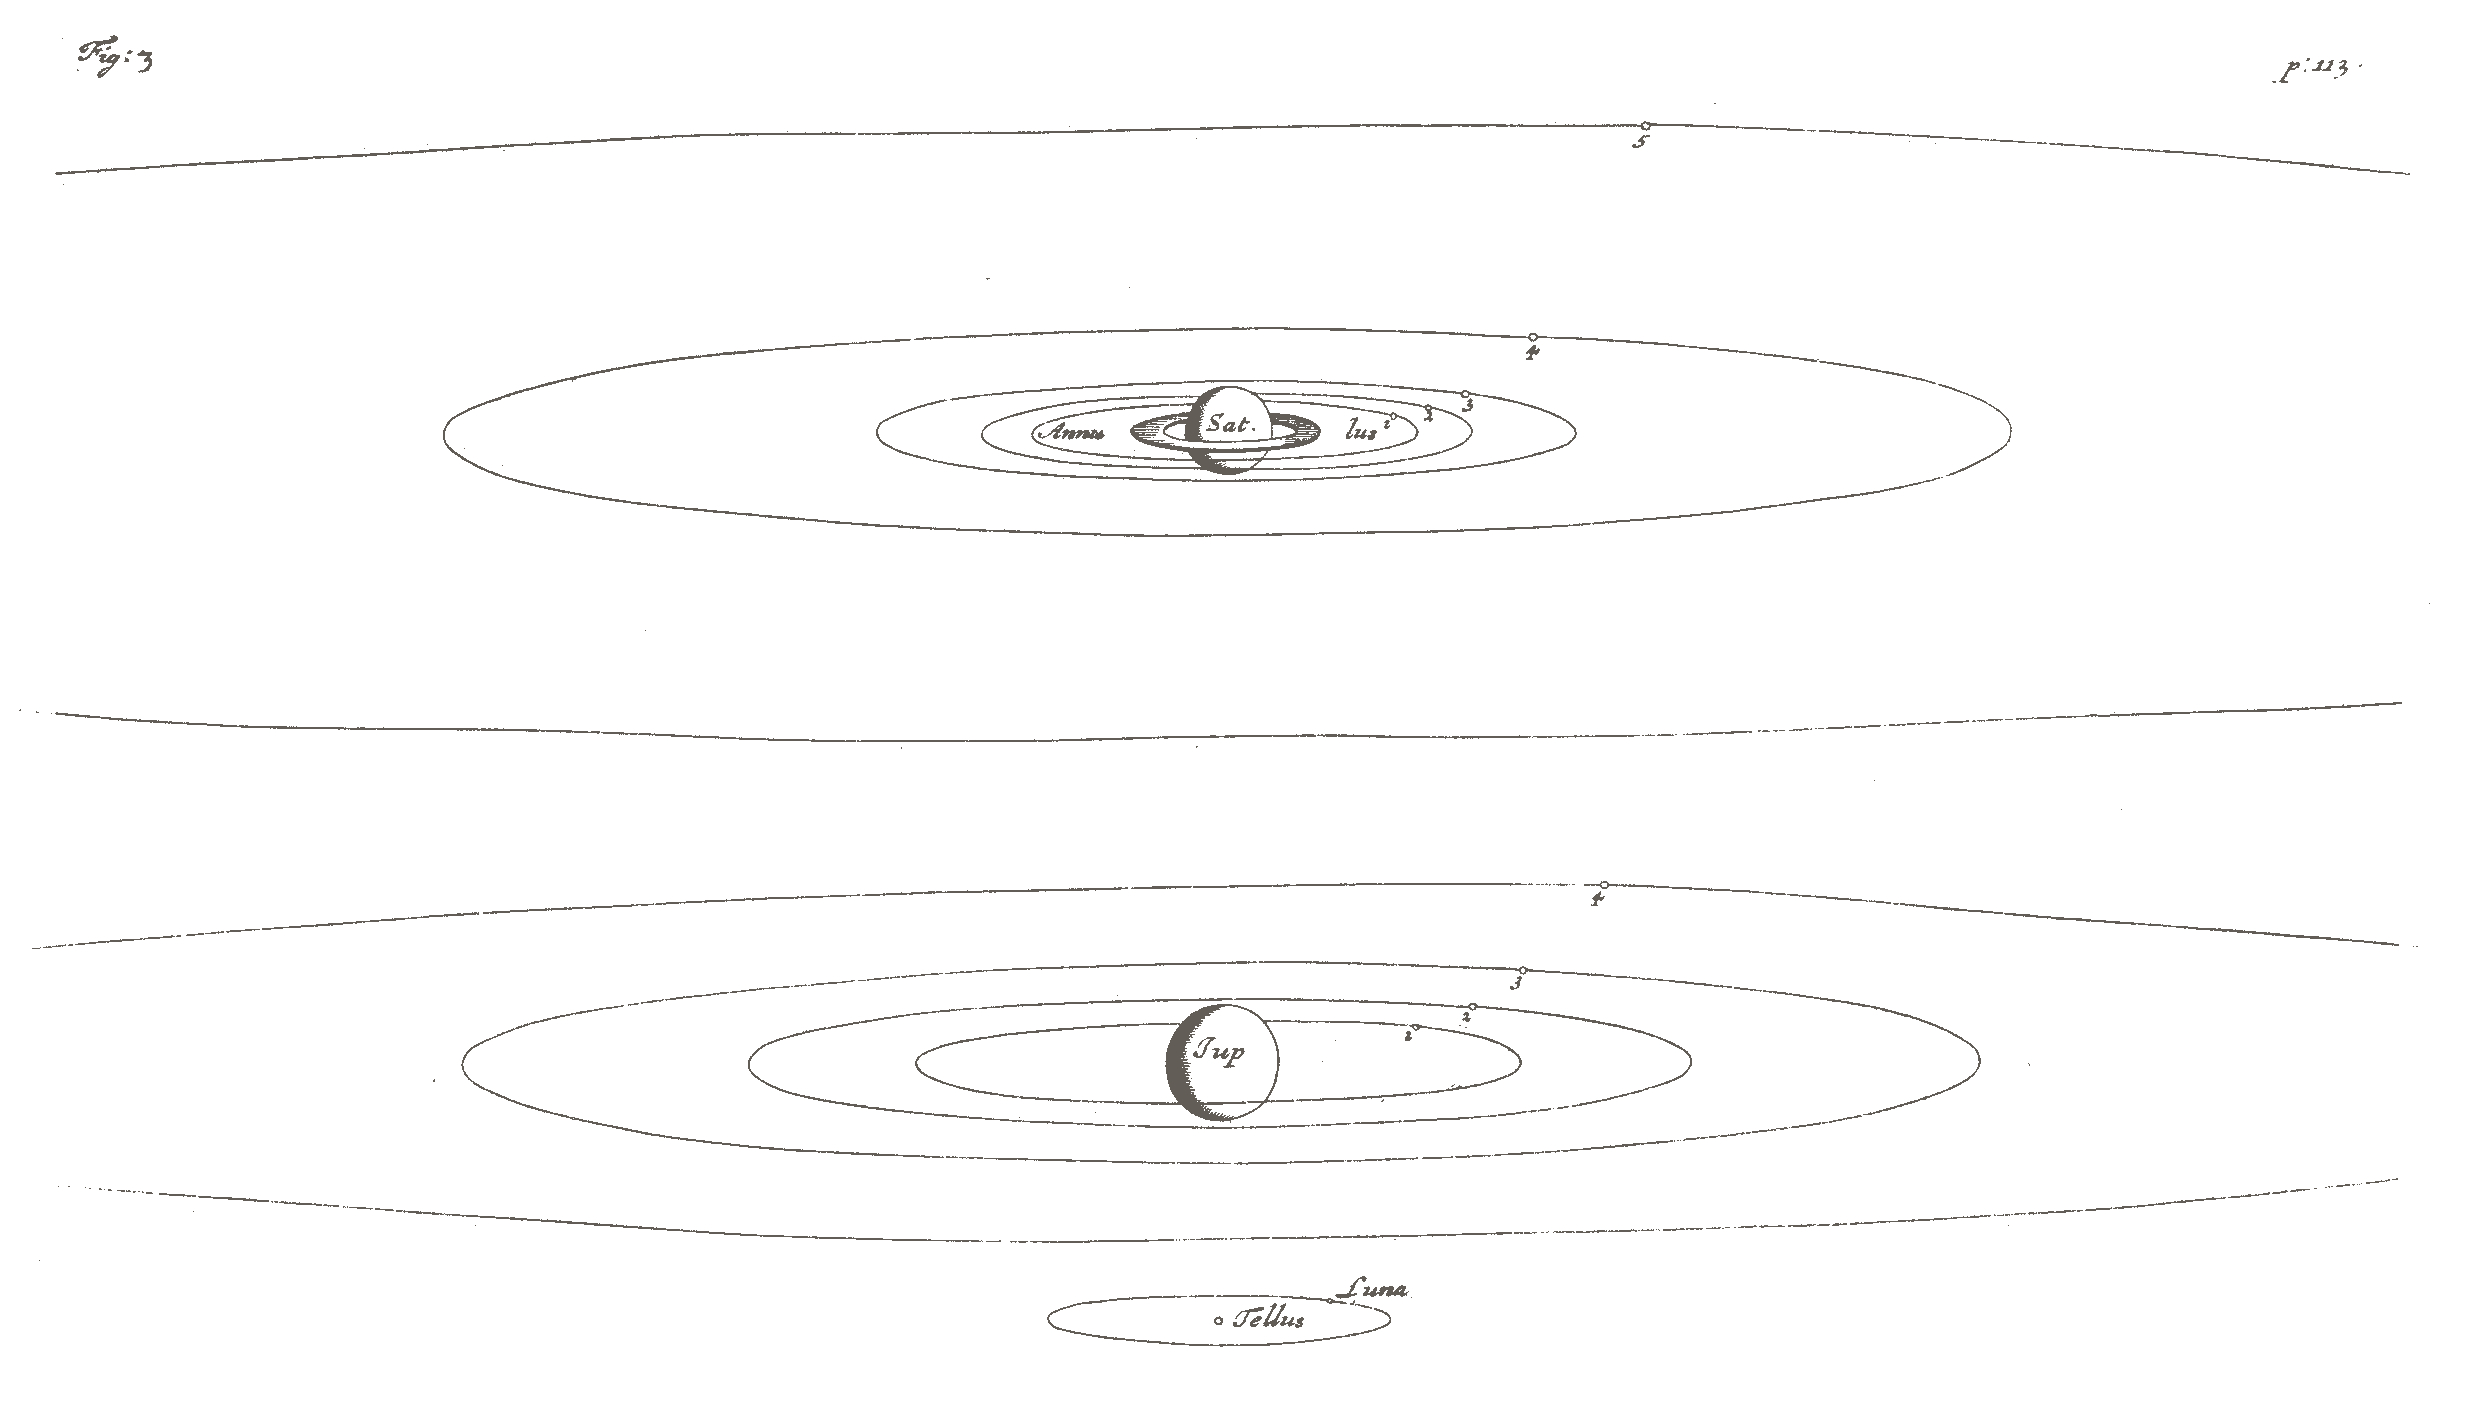
\includegraphics[width=.90\textwidth]{ct_3_en.jpg}
\end{center}

For the easier conception of their vast disparity, I have thought
fit [113] to add a Scheme of our Earth, with the Path of the Moon about it,
and the Globe of the Moon it self; and the Systems of Jupiter and Saturn,
where I have drawn every thing as near the true Proportion as possible.
Jupiter you see has his four, and Saturn his five Moons about him, all
plac'd in their Orbits. The Jovial we owe to Galilæo, 'tis well known: and
anyone may imagine he was in no small rapture at the discovery. The
outermost but one, and brightest of Saturn's, it chanc'd to be my lot, with a
Telescope not above 12 foot long, to have the first sight of in the year
1655. The rest we may thank the industrious Cassini for, who used the
Glasses of Jos.  Campanus's Work, first of 36, and afterwards of as many
above 100 foot long. He has often, and particularly in the year 1672, show'd
me the third and fifth. The first and second he gave me notice of by Letters
in the year 1684. but they are scarce ever to be seen, and I can't
positively say I had ever that happiness: but am as satisfied that they are
[114] there, as if I had; not in the least suspecting the Credit of that
worthy man. Nay, I am afraid there are one or two more still behind, and not
without reason. For between the fourth and fifth there's a distance not at
all proportionable to that between all the others: Here for ought I know may
lurk a sixth Gentleman; or perhaps there may be another without the fifth
that may yet have escaped us: for we can never see the fifth but in that
part of his Orbit, which is towards the West: for which we shall give you a
very good reason.  Perhaps when Saturn comes into the Northern Signs, and is
at a good height from the Horizon (for at the writing of this he is at his
lowest) you may happen to make some new Discoveries, good Brother, if you
would but make use of your two Telescopes of 170 and 210 foot long; the
longest, and the best I believe now in the World. For tho we have not yet
had an opportunity of observing the Heavens with them (as well by reason of
their unweildiness, as for [115] the interruption of our Studies by your
absence) yet I am satisfied of their Goodness by our trial of them one
night, in reading a Letter at a vast distance by the help of a Light. I
cannot but think of those times with pleasure, and of our diverting labour
in polishing and preparing such Glasses, in inventing new Methods and
Engines, and always pushing forward to still greater and greater things. But
to return to those Diagrams.



\section{The proportion of the Diameter of Jupiter, and of
the Orbs of his Satellites, to the Orbit of the Moon
round the Earth}

I have there made the Diameter of Jupiter about two third parts of our
distance from the Moon: for the Diameter of Jupiter is above twenty times
bigger than that of the Earth; which the distance of the Moon contains
about thirty times. The Orbit of the outermost of Jupiter's Guards is to
that of the Moon round the Earth, as 8 and ? is to 1. And each of these
Moons, by the shadow they make upon Jupiter, cannot be less than our
Earth.


\section{The periods of Jupiter's Moons}

Their Periods, that I may not omit them, are according to Cassini's account
these. That of the inmost is one day, 18 hours, 28 minutes, [116] and 36
seconds. The second spends 3 days, 13 hours, 13 min. 52 sec. in going
round him. The third 7 days, 3 hours, 59 min. 40 sec. The fourth 16 days,
18 hours, 5 min. 6 sec. The distance of the innermost from Jupiter himself
is 2 5/6 of his Diameters. That of the second is 4 and a half: Of the third 7
and one sixth part: Of the fourth 12 and two thirds, of the same Diameters.


\section{And Saturn's}

The innermost of Saturn's Guards moves round him in 1 day, 21 hours, 18 min.
31 sec. The second in 2 days, 17 hours, 41 min. 27 sec. The third in 4 days,
11 hours, 47 min. 16 sec. The fourth in 15 days, 22 hours, 41 min. 11 sec.
The fifth in 79 days, 7 hours, 53 min. 57 sec. Their distances from the
Center of Saturn are, that of the first almost one, that is 39 fortieth
parts of the Diameter of his Ring; that of the second one and a quarter of
those Diameters; of the third one and three quarters of them; of the fourth
four, or according to my calculation, but 3 and a half; of the fifth 12,
which were found with vast pains and labour.  [117] Now can any one took
upon, and compare there Systems together, without being amazed at the vast
Magnitude and noble Attendance of there two Planets, in respect of this
little pitiful Earth of ours? Or can they force themselves to think, that
the wise Creator has disposed of an his Animals and Plants here, has
furnish'd and adorn'd this Spot only, and has left all those Worlds bare and
destitute of Inhabitants, who might adore and worship him; or that all those
prodigious Bodies were made only to twinkle to, and be studied by some few
perhaps of us poor fellows?


\section{This proportion true according to all modern Observations}

I do not doubt but there will be some who will think we Romance very
much about the Magnitude of these Planets. For will you pretend to make
them who are taken up in admiring the largeness of this Globe, its multitude
of Nations, Cities, and Empires; can you pretend I say to make them ever
believe that there are Places in comparison of which the Earth is as incon-
siderable as my Figure would make it? No, they know better things [118]
they'l cry. But they may vouchsafe to be inform'd, that these Proportions
are those which the best Astronomers of this Age have agreed upon. For
if the Earth be distant from the Sun ten or eleven thousand of its own Di-
ameters, according to the accounts of Monsieur Cassini in France, and Mr.
Flamsted in England, wherein they made use of very exact Observations of
the Parallaxes of Mars; or if, according to a very probable Conjecture of
mine, it be distant twelve thousand, then the Magnitudes of the other Orbs
will very near answer the Proportions here settled.


\section{The apparent magnitude of the Sun in Jupiter, and a way of finding
what light they there enjoy}

But to return to Jupiter. The Sun appears to them five times less than to
us, and consequently they have but the five and twentieth part of the Light
and Heat that we receive from it. But that Light is not so weak there as we
imagine, as is plain by the brightness of that Planet in the Night; and that
when the Sun is so far eclips'd to us, as that the 25th part of his Disk be
not free from the Shadow, he is not sensibly darken'd. But if you have a
[119] mind exactly to know the quantity of light that Jupiter enjoys, you
may take a Tube of what length you please. Let one end of it be clos'd with a
Plate of Brass, or any such thing, in the middle of which there must be a
hole, whose breadth must have the same proportion to the length of the Tube,
as the Chord of 6 Minutes bears to the Radius; that is about as one is to
570.  Let the Tube be turn'd so to the Sun, that no Light may fall upon a
white Paper plac'd at the end of it, but what comes through the little hole
at the other end of the Tube. The Rays that come through this will represent
the Sun upon the Paper of the same Brightness that the Inhabitants of
Jupiter see it in a clear day. And if removing the Paper you place your eye
in the same place, you will see the Sun of the same Magnitude and Brightness
as you would were you in Jupiter.


\section{And in Saturn}

If you make the hole twice as little in breadth, you will see the same of
Saturn. And altho his Light be but the hundredth part of ours, yet you
[120] see it makes him shine finely in a dark night. But in cloudy days what
shall the poor Inhabitants do? Why if we were to be Judges but miserably,
but yet I warrant they do not at all complain. Perhaps they may be like
Owls and Bats, and may love the Twilight better than open day.


\section{In Jupiter their days are 5 hours}

But it's a little strange, that when Jupiter is so much bigger than our
Planet, their Days and Nights should be but five of our Hours. By this we
may see that Nature has not observ'd that proportion that their bulk seems
to require, seeing in Mars the days are very little different from ours. But
in the length of their years, that is in the revolution of the Planets round
the Sun, there is an exact proportion to their distances from the Sun
followed. For as the Cubes of their distances, so are the Squares of their
Revolutions, as Kepler first found out. Which proportion the Moons of
Jupiter and Saturn keep in their Courses round those.


\section{Always the same length}

As the Years and Days in Jupiter are different from ours in this respect, so
are the Days in another; [121] namely, that they are all of the same length.
For they there enjoy a perpetual Equinox, their Axis having little or no
inclination to their Orbit, as the Earth's has, as has bin discover'd by
Telescopes. The Countries that lie near their Poles have little or no heat,
by reason the Rays of the Sun fall so obliquely upon them; but then they are
freed from the Inconveniency that ours are troubled with, of tedious long
half-year Nights, and have the constant returns of Day and Night every
five hours. Indeed we should not be contented with such short days, and
should count our selves very ill dealt with if we had not twice as long, tho
upon no other account, but that what is our own, to be sure, must be best.
The rest of the Planets are so near the Sun, (Mars himself never being above
18 degrees from it) that in Jupiter they have the sight only of Saturn.  But
we cannot deny but that their four Moons stand them in greater stead than
our one doth us, if 'twere only that they seldom know any such thing as to
be without Moonshiny [122] Nights. And they are of great advantage to them,
as we said before, in their Navigation, if they have any such thing. Not to
mention the pleasant sights of their frequent Conjunctions and Eclipses,
things that they are seldom a day without.  Saturn enjoys all those
Pleasures and Advantages in a still higher degree, as well for his five
Moons, as for the delightful prospect that the Ring about him affords his
Inhabitants night and day. But we will be as kind to them as we have bin to
the rest of the Planets, in giving an account of their Astronomy.


\section{They see the fixt Stars just as we do}

And first of all we shall observe what we might have remark'd before, but
will be more strange here, that the fix'd Stars appear to them of the same
Figure and Magnitude, and with the same degree of Light that they do to us:
and this, by reason of their immense distance, of which we shall have
occasion to speak by and by. In comparison with which the space that a
Bullet shot out of a Cannon could travel in 25 years, would be almost
nothing.  [123] Their Astronomers have all the same Signs of the Bear, the
Lion, Orion, and the rest, but not turning upon the same Axis with us: for
that's different in all the Planets.  As Jupiter can see no Planet but
Saturn, so Saturn knows of no Planet but Jupiter; which appears to him much
as Venus doth to us, never removing above 37 degrees from the Sun. The
length of their days I cannot determine: But if from the distance and period
of his innermost Attendant, and comparing it with the innermost of
Jupiter's, a Man may venture to give a guess, they are very little different
from Jupiter's, 10 hours or somewhat less. But whereas in Jupiter there are
equally divided between Light and Darkness, the Saturnians must perceive a
more sensible difference than we, especially between Summer and Winter. For
our Axis inclines to the place of the Ecliptick but 23 degrees and a half,
but there's above 31. Upon this account his Moons must decline very much
from the Path that the Sun seems to move [124] in, and his Inhabitants can
never have a full Moon but just at the Equinoxes: two of which fall out in
30 of our years. 'Tis this Position of the Axis too that is the cause of
those delightful appearances, and wonderful prospects that its Inhabitants
enjoy: for the better understanding of which I shall draw a Figure of Saturn
with his Ring about him: in which the proportion between the Diameters of
the Globe and Ring is as 9 to 4.  And the empty space between them is of the
same breadth with the Ring it self. All Observations conspire to prove that
that is of no great thickness, altho if we should allow it six hundred
German Miles, I think, considering its Diameter, we should not overdo the
matter.  

\begin{center}
	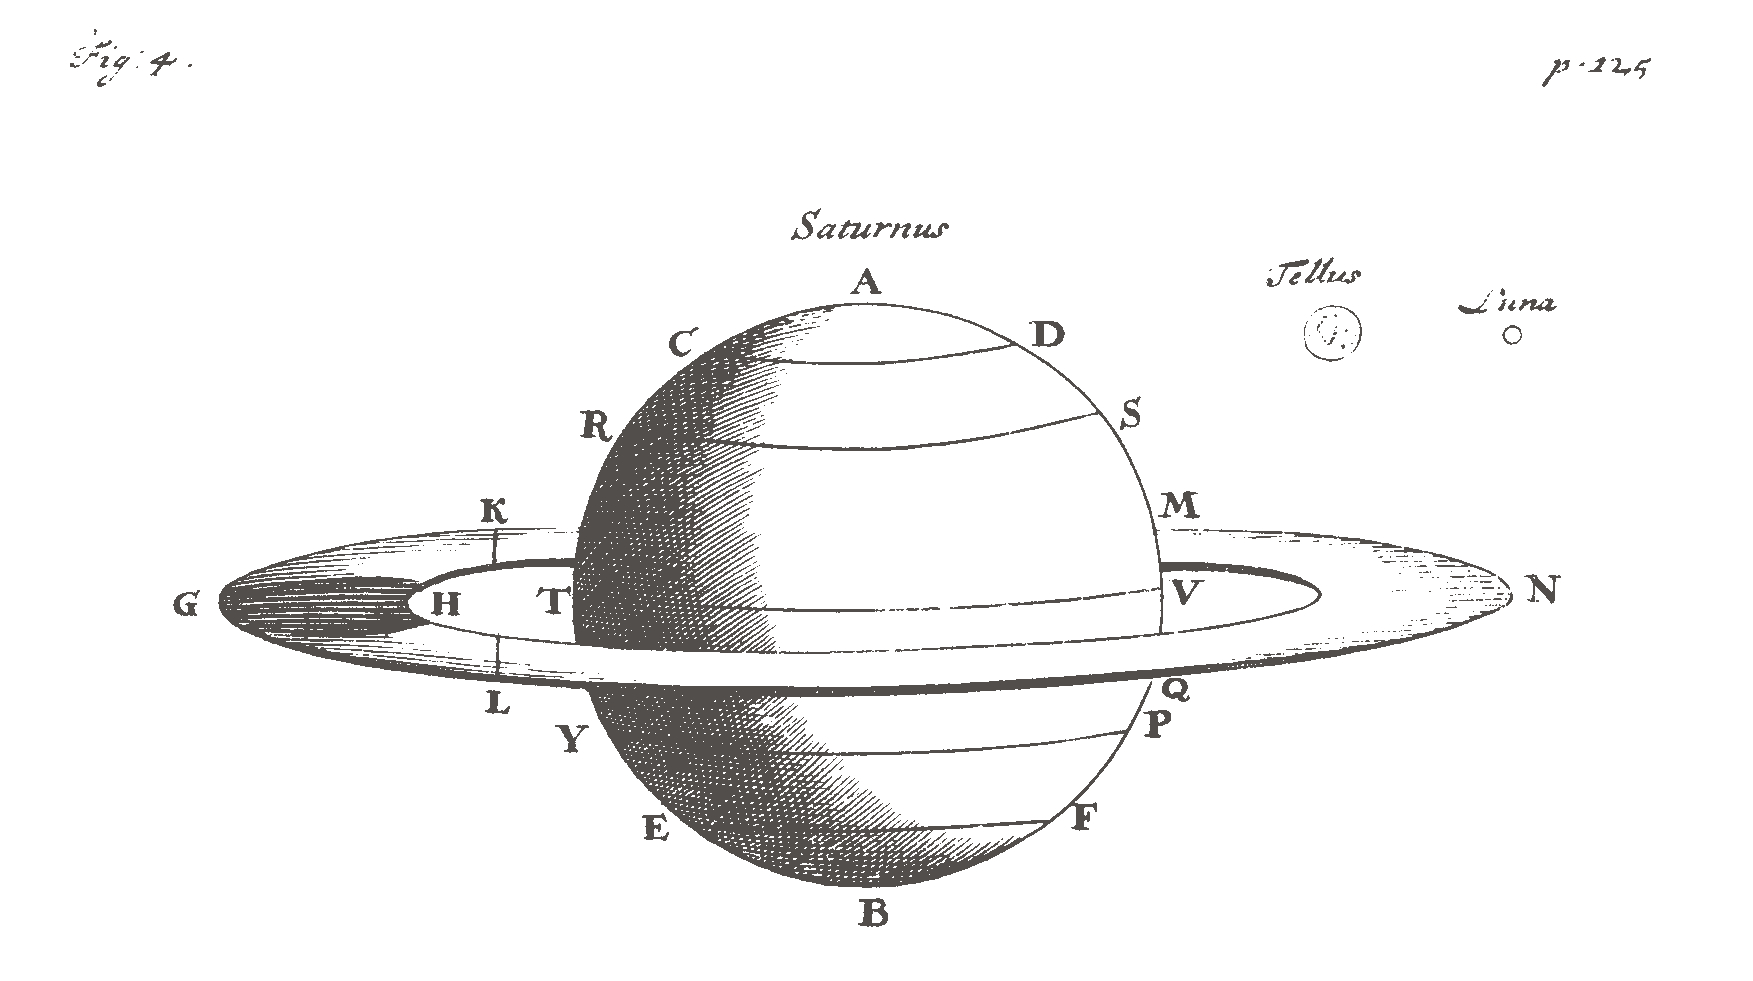
\includegraphics[width=.90\textwidth]{ct_4_en.jpg}
\end{center}

Suppose then that to be the Globe of Saturn, whose Poles are A, B.
GN es the Diameter of the Ring, as you view it sideways, representing a
narrow Oval. Those that live about the Poles within the Arches CAD, EBF,
each of which are 54 degrees, (if the Cold will suffer any body to live
[125] there) never have a sight of the Ring.


\section{The appearances of the Ring in Saturn}

From all other parts it is continually to be seen for fourteen years and
nine Months, which is just: half their year. The other half it is hid from
their view. Those then that dwell between the Polar Circle CD, and the
Equator TV, all that time that the Sun enlightens the part opposite to them,
have every night the sight of a piece of it HGL, much in the shape of a
shining Bow, which comes from the Horizon, but is darken'd in the middle by
the shadow of Saturn GH, which reaches most commonly to the outermost rim of
it. But after midnight that Shadow by little and little begins to move
towards the right hand to those in the Northern, but the left to those in
the Southern Hemisphere. In the morning it disappears, leaving behind it a
likeness indeed of a Bow, but much paler and weaker than our Moon is in the
day-time. For they, as I said before, have an Atmosphere, or an Air
surrounding them enlighten'd by the Sun. Otherwise Night and Day they would
have their Ring, [126] their Moons, and all the fix'd Stars, equally
conspicuous. Another thing that must make the sight of their Ring very
curious, is, that by some Spots in it, it is discover'd to turn round upon
it self: A thing that those that are so near cannot but take notice of, when
we that live at this distance can descry a great Inequality, the inside of
it being brighter much than the outside is. When the shadow of the Globe
falls upon that part of the Ring GH, the shadow of the Ring at the same time
darkens another part of the Globe about PF, which otherwise would have the
Sun upon it. So that there is always a Zone of the Globe PYFE, sometimes of a
larger extent than at others, which is depriv'd of the sight both of the Sun
and Ring for a considerable time, the latter of which hides some, part of
the Stars from it too. An amazing thing it must be, all of a sudden to have
the Sun darken'd, and, fall into a pitch-night, without seeing any cause of
such an accident. All which while their Moons are their only Comfort.  The
other half of the [127] year the Hemisphere TBV enjoys the same Light that
TAU before did, and then this undergoes those long Eclipses that that before
suffer'd. At the Equinoxes, when the Sun is in the same Plane with the Ring,
the Saturnians cannot well perceive it: no not even we with our Glasses, by
reason of its Darkness. This happens when Saturn, viewed from the Sun, is
advanced one and twenty degrees and a half in Virgo or Pisces, as I show'd
formerly in my System of Saturn: Where there is an account given of the
Risings of the Sun above the Ring, throughout all the Saturnian Year.  With
Saturn in this Scheme you have the Globes of the Earth and Moon drawn in
their true proportion, to put you in mind again of a thing very fit to be
remember'd, how very small our Habitation is when compar'd with that Globe
or the Ring about it. And now anyone, I suppose, can frame to himself a
picture of the Night in Saturn, with two Arches of the Ring, and five Moons
shining [128] about, and adorning him. This then shall be what I have to say
to the primary Planets.  We are now come a little lower, to make an enquiry
into the Attendants of there Planets, especially our own. And here we shall
meddle not only with their Astronomy, but shall also search into their
Furniture and Ornament, if they are found to have any such thing, which we
have put off considering till now.


\section{Very little to be said of the Moon}

And here one would think that when the Moon is so near us, and by the
means of a Telescope may be so nicely and exactly observ'd; it should af-
ford us matter for more probable Conjectures than any of the other remote
Planets. But it is quite otherwise, and I can scarce find any thing to say
of it, because I have not a Planet of the same nature before my eyes, as in
all the primary ones I have. For they are of the same kind with our Earth;
and seeing all the Actions, and every thing that is here, we may make a
reasonable Conjecture at what we cannot see in those Worlds.
[129]


\section{The Guards of Jupiter and Saturn of the same nature with our Moon}

But this we may venture to say, without fear, that all the Attendants of
Jupiter and Saturn are of the same nature with our Moon, as going round
them and being carry'd with them round the Sun just as the Moon is with
the Earth. Their Likeness reaches to other things too, as you'l see by and
by. Therefore whatsoever we can with reason affirm or fancy of our Moon
(and we may say a little of it) must be suppos'd with very little alteration
to belong to the Guards of Jupiter and Saturn, as having no reason to be
at all inferior to that.


\section{The Moon hath Mountains}

The Surface of the Moon then is then found, by the least Telescopes of
about three or four foot, to be diversified with long Tracts of Mountains,
and again with broad Valleys. For in those parts opposite to the Sun you
may see the Shadows of the Mountains, and often discover the little round
Valleys between them, with a hillock or two perhaps rising out of them.
Kepler from the exact roundness of them would prove that they are some
vast work of the rational [130] Inhabitants. But I can't be of his mind, both
for their incredible largeness, and that they might easily be occasion'd by
natural Causes.


\section{But no Sea, nor Rivers, nor Clouds, nor Airs and Waters}

Nor can I find any thing like Sea there, tho he and many others are of the
contrary opinion I know. For those vast Countries which appear darker than
the other, commonly taken for and call'd by the names of Seas, are discver'd
with a good long Telescope, to be full of little round Cavities; whose
Shadow falling within themselves, makes them appear of that colour: and
those large Champains there in the Moon you will find not to be always even
and smooth, if you look carefully upon them: neither of which two things can
agree to the Sea. Therefore those Plains in her that seem brighter than the
other parts, must consist, I suppose, of a whiter sort of Matter than they.
Nor do I believe that there are any Rivers, for if there were, they could
never escape our sight, especially if they run between the Hills as ours
do.  Nor have they any Clouds to furnish the Rivers with [131] Water. For if
they had, we should sometimes see one part of the Moon darken'd by them, and
sometimes another, whereas we have always the same prospect of her.  'Tis
certain moreover, that the Moon has no Air or Atmosphere surrounding it as
we have. For then we could never see the very outermost Rim of the Moon so
exactly as we do, when any Star goes under it, but its Light would terminate
in a gradual faint shade, and there would be a sort of a down as it were
about it; not to mention, that the Vapors of our Atmosphere consist of
Water, and consequently that where there are no Seas or Rivers, there can be
no Atmosphere. This is that notable difference between that Planet and us
that hinders all probable Conjectures about it. If we could but once be sure
that they had Water, we might come to an Agreement, and plant a Colony
perhaps there; we might allow it then most of our other Privileges, and,
with Xenophanes, furnish it with Inhabitants, Cities, and Mountains. But as
'tis, I [132] cannot imagine how any Plants or Animals, whose whole
nourishment comes from liquid Bodies, can thrive in a dry, waterless,
parch'd Soil.


\section{The Conjecture of its Plants and Animals very dubious}

What then, shall this great Ball be made for, nothing but to give us a little
puny light in the Night-time, or to raise our Tides in the Sea? Shall not
we plant some People there that may have the pleasure of seeing our Earth
turn upon itself, presenting them some times with a prospect of Europe and
Africa, and then of Asia and America; sometimes half, and sometimes full?
What! and must all those Moons round Jupiter and Saturn be condemn'd
to the same uselesness? I do not know what to think of it, because I know
of nothing like them to found a Conjecture upon. And yet 'tis not improb-
able that those great and noble Bodies have somewhat or other growing
and living upon them, tho very different from what we see and enjoy here.
Perhaps their Plants and Animals may have another sort of Nourishment
there. Perhaps the moisture of the Earth there is but just sufficient [133]
to cause a Mist or Dew, which may be very sutable to the growth of their
Herbs. Which I remember is Plutarch's opinion, in his Dialogue upon this
Subject. For in our Earth a very little Water drawn from the Sea into Dew,
and falling down again upon the Herbs, would be sufficient for all our needs,
without any Rain or Showers.


\section{Jupiter's and Saturn's Moons turn always the same side to them}

But these are mere guesses, or rather doubts, but yet they are the best we
can make of this, and all those other Moons: for, as I said before, they are
all of the same nature, which is proved likewise by this, that as our Moon
can afford us the sight never but of one side of her, so they turn always
the same face to their primary Planets. You wonder, I suppose, how we came
to know so much; but 'twas no hard matter, after that Observation which I
just now made, that the outermost of Saturn's Moons can never be seen but
when she is on the West-side of her Planet. The reason of which is plainly
this, that one side of her is darker, and does not reflect the Light so much
as the other, [134] which when it is turned towards us, we cannot see by
reason of its weak Light. This always happening when 'tis East of him, and
never on the other side, is a manifest proof that she always keeps the same
side toward Saturn. Now since the outermost of Saturn's and our Moon carry
themselves thus to the Planets round which they move, who can well doubt it
of all the rest round Jupiter and Saturn? And there's a very good reason for
it, namely, that the matter of which those Moons consist, being heavier, and
more solid on the side that is averse from us, than on that which we have
the sight of, does consequently fly with a greater force from the Centre of
its Motion: for otherwise, according to the Laws of Motion, it should turn
the same side always, not to its Planet; but to the same fixt Stars.  This
Position of the Moons, in respect of their Planets, must occasion great many
very pretty, wonderful sights to their Inhabitants, if they have any: which
is very doubtful, but may for the present be suppos'd.  [135]


\section{The Astronomy of the Inhabitants of the Moon}

An enquiry into our Moon may serve for all the rest. Its Globe is divided
into two parts, after that manner, that those who live on one side never
lose the sight of us, and those on the other never enjoy it. Only those who
live on the Confines of each of these lose us, and see us again by turns. The
Earth to them must seem much larger than the Moon doth to us, as being in
Diameter above four times bigger. But the best of it is, that night and day
they see it always in the very same part of the Heaven, as if it never moved:
some of them as if 'twas falling upon their heads: others somewhat above
the Horizon, and others always in the Horizon, still turning upon it self, and
presenting them every twenty four hours with a view of all its Countries,
even of those that lie near the Poles (I could wish my self in the Moon only
for the sight of them) yet unknown and undiscover'd by us. They have it
in its monthly Wane and Increase, they see it half, and horned, and full, by
turns, just as we do their Planet. But the Light [136] that they borrow of us
is five times larger than what they pay us again. So that in dark nights that
part that hath the advantage of being towards us, receives a very glorious
Light, tho let Kepler say what he will, no Heat from us. Their Days are
always of the same length with their Nights; and the Sun rising and setting
to them but once in one of our Months, makes the time both of their Light
and Darkness to be equal to 15 of our days. If their Bodies are of the same
Metal with ours, those that have the Sun pretty high in their Horizon, must
be like to be burnt up in such long days. For the Sun is not farther from
them than he is from us. This will be the case of those that live upon the
Borders of the two Hemispheres we talk'd of; but those that live under the
Poles of the Moon will be just about as hot as our Whale-Fishers about
Island and Nova Zemla are, in the Summer-time: who are in so little danger
of being roasted, that in the middle of their Summer, in their days of three
Months length, they are ready to lose their [137] fingers ends. The Poles
of the Moon I call those, round which the fixt Stars seem to turn to its
Inhabitants, which are different from ours, and those of the Ecliptick, altho
they move round these latter, at the distance of five degrees, in a period
of nineteen Years. Their Year they count by the Motion of the Stars, and
their return to the Sun, and 'tis the same with ours. They can easily do it,
because they have the Stars day and night, notwithstanding the Light of the
Sun: for they have no Atmosphere (which is the only reason that we don't
every day enjoy the same sight) to hinder their Observations. Nor have
they any Clouds to obstruct their view, so that they have an easier work
than we to find out the Courses, but a more difficult to make a true System
of the Planets. For they will be apt to lay a wrong Foundation upon the
Immobility of the Earth, which will lead them into more dangerous Errors
than ever it did us.


\section{This may be applied to the Moons about Jupiter and Saturn}

All that I have said belongs as well to Jupiter's and Saturn's as to our Moon
in respect of [138] the Planets they move round. The length of their Day and
Night is always equal to the time of their Revolution: for example, the fifth
Moon moves round Saturn in 80 days, and the days and nights there are equal to
forty of ours. Both their Summer and Winter (Saturn moving round the Sun in
thirty years) are fifteen years long. Therefore it is impossible but that their
way of living must be very different from ours, having such tedious Winters,
and such long watching and sleeping times.  Having thus explain'd the primary
and secondary Planets round the Sun, we should next set about the third sort,
the Sun and fixt Stars; but before we do that, it will be worth while to set
before you at once, in a clearer and more plain Method than hitherto, the
Magnificence and Fabrick of the Solar System. Which we can't possibly do in so
small a space as one of our Leaves will but admit of, because the Bodies of the
Planets are so prodigiously small in comparison of their Orbs. But what is
wanting in Figure shall be [139] made up in Words. Going back then to the first
Scheme, suppose another like it, and proportionable, drawn upon a very large
smooth Plain; whose outermost Circle representing the Orb of Saturn, must be
conceived three hundred and sixty foot in Semi-diameter. In which you must
place the Globe and Ring of Saturn of that bigness as the 2d Figure shows you.
Let all the other Planets be supposed everyone in his own Orbit, and in the
middle of all the Sun, of the same bigness that that Figure represents, namely,
about four inches in Diameter. And then the Orbit or Circle in which the Earth
moves, which the Astronomers call the magnus Orbis, must have about six and
thirty foot in Semidiameter. In which the Earth must be conceived moving, not
bigger than a grain of Millet, and her Companion the Moon scarcely perceivable,
moving round her in a Circle a little more than two Inches broad, as in the
Figure here adjoined, where the line AB represents a small portion of that
Circle which the Earth moves in: [140] the small Circle therein C is the Earth
and the Circle DE the path of the Moon round it, in which the body of the Moon
is D.  

\begin{center}
	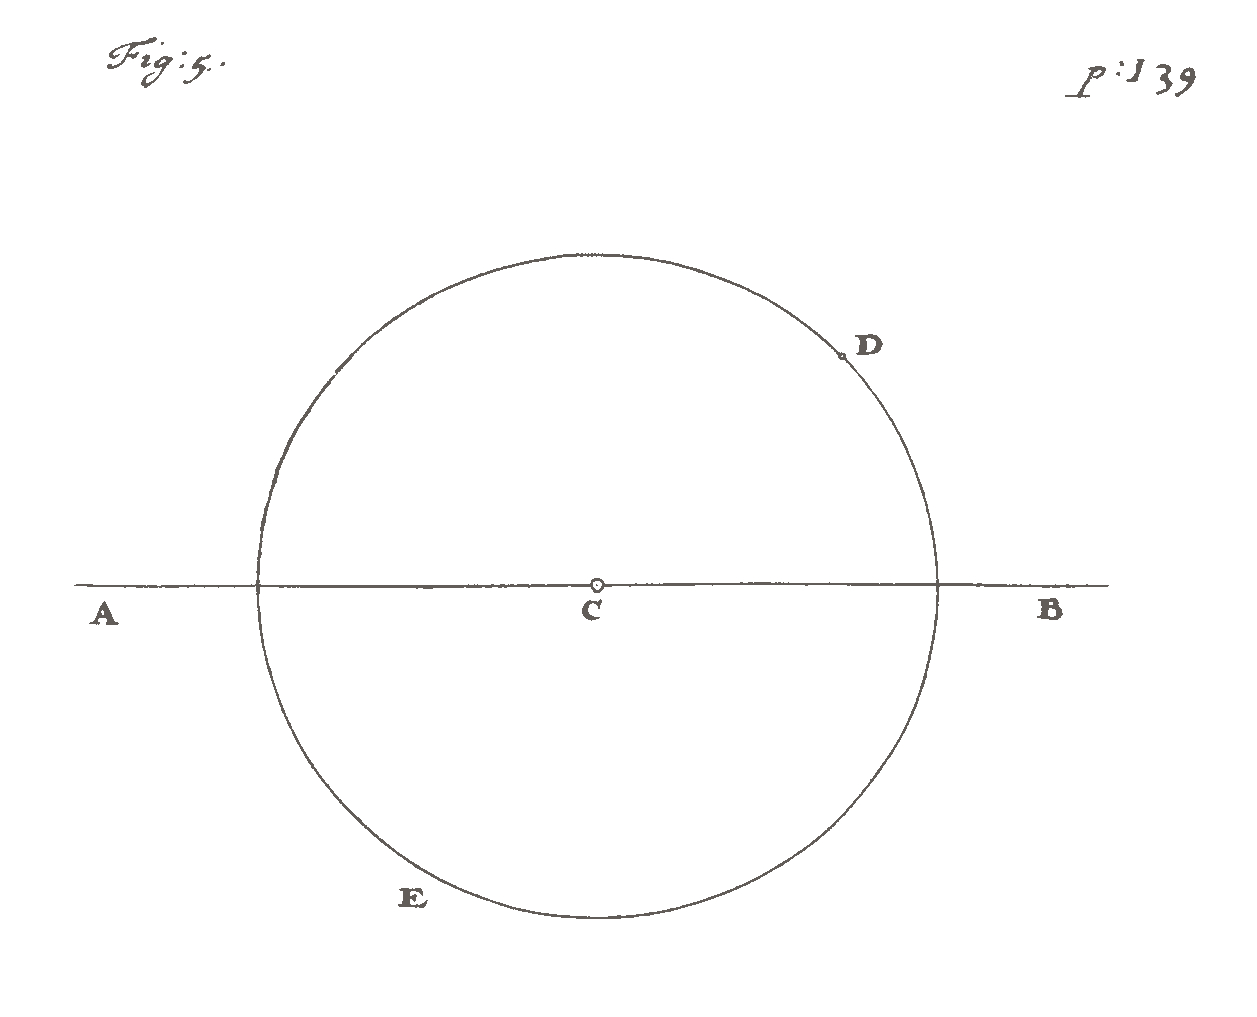
\includegraphics[width=.90\textwidth]{ct_5_en.jpg}
\end{center}

The outermost of Saturn's Moons move in an Orbit whose Semidiameter is
29 inches; that of Jupiter in a somewhat smaller, whose Semidiameter is 19 and
a quarter.  And thus we have a true and exact Description of the Sun's Palace,
where the Earth will be twelve thousand of its Semidiameters distant from him,
which in German Miles makes above seventeen Millions. But perhaps we may have a
clearer comprehension of this vast length, by comparing it with some very swift
Motion. 'Twas a pretty fancy of Hesiod, that an Anvil let fall from the top of
Heaven, reach'd the Earth the tenth day of its Journey, and in ten more arriv'd
at the bottom of Hell, the end of it: so making the Earth the midway between
Heaven and Hell. I shan't make use of the Anvil, but of one as good, namely, a
Bullet shot out of a great Gun, which may travel per[141]haps in a moment, or
pulse of an Artery, about a hundred Fathom, as is prov'd by those Experiments
that Mersennnus in a Treatise of his relates; wherein the Sound was found to
extend it self eighty hundredth parts in that time.


\section{The immense distance between the Sun and the Planets illustrated}

I say then, that supposing a Bullet to move with this swiftness from the
Earth to the Sun, it would spend 25 years in its passage. To make a Journey
from Jupiter to the Sun, would require 125, and from Saturn thither 250
years. This account depends upon the measure of the Earth's Diameter,
which, according to the accurate Observations of the French, is 6 538 594
times six Paris feet, one degree being 57 060 of that measure. This shows
us how vast those Orbs must be, and how inconsiderable this Earth, the
Theatre upon which all our mighty Designs, all our Navigations, and all our
Wars are transacted, is when compared to them. A very fit Consideration,
and matter of Reflection, for those Kings and Princes who sacrifice the Lives
of so many People, only to flatter their Ambition in being [142] Masters of
some pitiful corner of this small Spot. But to return to the matter in hand,
now we have given you an account of the Sun's proportion to those Orbs
and Bodies, we'll see what more we can say of him.


\section{No ground for Conjecture in the Sun}

And there are some that have bin so civil, as to allow the Sun himself his
Inhabitants. But upon what reason I cannot imagine, there being less
ground for a probability in him than in the Moon. For we are not yet sure,
whether he be a compact or liquid Globe; altho, if my account of Light be
true, upon that account I should rather think him liquid: which his
roundness and equal distribution of his Light to all parts are an Argument
for. For that inequality on his Surface, which is discover'd by the
Telescopes, (and that not always neither) which makes men fancy boiling Seas
and belching Mountains of Fire, is nothing but the trembling Motion of the
Vapors our Atmosphere is full of near the Earth; which is likewise the cause
of the Stars twinkling.


\section{The Faculæ in the Sun not easily seen}

Nor could I ever have the luck to discern those [143] bright Spots they brag
so much of in the Sun as well as of his dark ones, tho the latter I have very
often seen; so that with very good reason I can doubt whether there's any
such thing. For, in all the exact Observations, I could never find any such
pretended to be seen any where but just about his dark Spots; and it is no
great wonder that those Parts which are so near the darker, should appear
somewhat brighter than the rest.


\section{By reason of its Heat no Inhabitants like ours can live in the Sun}

That the Sun is extremely hot and firy, is beyond all dispute, and such
Bodies as ours could not live one moment in such a Furnace. We must make new
sort of Animals then, such as we have no Idea or Likeness of among us, such
as we can neither imagine nor conceive: which is as much as to say, that
truly we have nothing at all to say. No doubt that glorious and vast Body
was made for some noble end and use, and fram'd with excellent design.  And I
think we all very well know and feel its Usefulness in that effusion of
Light and Heat to all the Planets round it; in the preservation and
happiness of all [144] living Creatures, and that not only in our Ball, but
in those vast Globes of Jupiter and Saturn, not much inferior to its own.
These are such great, such wise ends, that it is not strange that the Sun
should have bin made, if it had bin only upon their account. For, as for
Kepler's fancy, that he hath another Office, namely, to help on the Motion
of the Planets in their own Orbs, by turning them round their Axis, (which
he would fain establish in his Epitome) I shall give good Reasons why I
cannot assent to it.


\section{The fix'd Stars so many Suns}

Before the invention of Telescopes, Stars so it seem'd to contradict Coper-
nicus's Opinion, to make the Sun one of the fix'd Stars. For the Stars of
the first Magnitude being esteemed to be about three minutes Diameter; and
Copernicus (observing that tho the Earth changed its place, they always kept
the same distance from us) having ventur'd to say that the Magnus Orbis was
but a point in respect of the Sphere in which they were placed, it was a
plain consequence that everyone of them that appeared any thing bright, must
[145] be larger than the Path or Orbit of the Earth: which is very absurd.
This is the topping Argument that Tycho Brahe set up against Copernicus. But
when the Telescopes shav'd them of their fictitious Rays, and show'd 'em to
us bare and naked (which they do best when the Eye-glass is black'd with
Smoke) just like little shining Points, then that difficulty vanished, and
the Stars might still be Suns. Which is the more probable, because their
Light is certainly their own: for it's impossible that ever the Sun should
send, or they reflect it at such a vast distance. This is the opinion that
commonly goes along with Copernicus's System.


\section{They are not all in the same Sphere}

And the Patrons of it do also with reason suppose, that all these Stars are
not in the same Sphere, as well because there's no Argument for it, as that
the Sun, which is one of them, cannot be brought to this Rule. But it's
more likely they are scatter'd and dispersed all over the immense spaces of
the Heaven, and are as far distant perhaps from one another, as the nearest
of them are from the Sun.
[146] Here again too I know Kepler is of another opinion in his Epitome
of Copernicus's System, that we mention'd above. For tho he agrees with
us, that the Stars are diffus'd through all the vast Profundity, yet he cannot
allow that they have as large an empty space about them as our Sun has.
For at that rate, 'twas his opinion, we should see but very few, and those of
very different Magnitudes: For, seeing the largest of all appear so small to
us, that we can scarce observe or measure them with our best Instruments;
how must those appear that are three or four times farther from us? Why,
supposing them no larger than these, they must seem three or four times
less, and so on till a little farther they will not be to be seen at all: Thus we
shall have the sight of but very few Stars, and those very different one from
another; Whereas we have thousands, and those not considerably bigger or
less than one another. But this by no means proves what he would have
it; and his mistake was chiefly, that he did not consider the nature of Fire,
which makes it be seen at such [147] distances, and at such small Angles as
all other Bodies would totally disappear under. A thing that we need go no
farther than the Lamps set along the Streets to prove. For altho they are
a hundred foot from one another, yet you may count twenty of them in a
continued row with your eyes, and yet the twentieth of them scarce makes
an Angle of six Seconds. Certainly then the glorious Light of the Stars must
do much more than this; so that it's no wonder we should see a thousand
or two of them with our bare eyes, and with a Telescope discover twenty
times that number. But Kepler had a private design in making the Sun
thus superior to all the other Stars, and planting it in the middle of the
World, attended with the Planets: a favor that he did not desire to grant
the rest. For his aim was by it to strengthen his Cosmographical Mystery,
that the distances of the Planets from the Sun are in a certain proportion
to the Diameters of the Spheres that are inscrib'd within, and circumscrib'd
about Euclid's Polyedrical Bodies. [148] Which could never be so much as
probable, except there were but one Chorus of Planets moving round the
Sun, and so the Sun were the only one of his kind.
But that whole Mystery is nothing but an idle Dream taken from Pythago-
ras or Plato's Philosophy. And the Author himself acknowleges that the
Proportions do not agree so well as they should, and is fain to invent two or
three very silly excuses for it. And he uses yet poorer Arguments to prove
that the Universe is of a spherical Figure, and that the number of the Stars
must necessarily be finite, because the Magnitude of each of them is so.
But what is worst of all is, that he settles the space between the Sun and
the concavity of the Sphere of the fix'd Stars, to be six hundred thousand
of the Earth's Diameters. For this very good reason, forsooth, that as the
Diameter of the Sun is to that of the Orbit of Saturn, which he makes to be
as 1 to 2000, so is this Diameter to that of the Sphere of the fix'd Stars. A
mere fancy without any shadow of [149] Reason. I cannot but wonder how
such things as these could fall from so ingenious a Man, and so great an
Astronomer. But I must give my Vote, with all the greatest Philosophers of
our Age, to have the Sun of the same nature with the fix'd Stars. And this
will give us a greater Idea of the World, than all those other Opinions.


\section{The Stars have Planets about them like our Sun}

For then why may not every one of these Stars or Suns have as great a
Retinue as our Sun, of Planets, with their Moons, to wait upon them? Nay
there's a manifest reason why they should. For let us fancy our selves
placed at an equal distance from the Sun and fix'd Stars; we should then
perceive no difference between them. For, as for all the Planets that we now
see attend the Sun, we should not have the least glimpse of them, either
that their Light would be too weak to affect us, or that all the Orbs in
which they move would make up one lucid point with the Sun. In this station
we should have no occasion to imagine any difference between the Stars, and
should make no doubt if we [150] had but the sight, and knew the nature of
one of them, to make that the Standard of all the rest. We are then plac'd
near one of them, namely, our Sun, and so near as to discover six other
Globes moving round him, some of them having others performing them the same
Office.  Why then shall not we make use of the same Judgment that we would
in that case; and conclude, that our Star has no better attendance than the
others?  So that what we allow'd the Planets, upon the account of our
enjoying it, we must likewise grant to all those Planets that surround that
prodigious number of Suns. They must have their Plants and Animals, nay and
their rational ones too, and those as great Admirers, and as diligent
Observers of the Heavens as our selves; and must consequently enjoy
whatsoever is subservient to, and requisit for such Knowlege.  What a
wonderful and amazing Scheme have we here of the magnificent Vastness of the
Universe! So many Suns, so many Earths, and every one of them stock'd with
so many [151] Herbs, Trees and Animals, and adorn'd with so many Seas and
Mountains! And how must our wonder and admiration be encreased when we
consider the prodigious distance and multitude of the Stars?  That their
distance is so immense, that the space between the Earth and Sun (which is
no less than twelve thousand of the former's Diameters) is almost nothing
when compar'd to it, has more Proofs than one to confirm it. And this among
the rest, If you observe two Stars near one another, as for example those in
the middle of the Great Bears Tail, differing very much from one another in
Clearness, notwithstanding our changing our Position in our Annual Orbit
round the Sun, and that there would be a Parallax were the Star which is
brighter nearer us than the other, as is very probable it is, yet whatever
part of the year you look upon them, they will not in the least have altered
their distance. Those that have hitherto undertook to calculate their
Distance, have not bin able perfectly to [152] compass their design, by
reason of the extreme niceness and almost impossibility of the Observations
requisite for their purpose. The only Method that I see remaining, to come
at any tolerable probability in so difficult a case, I shall here make use
of. Seeing then that the Stars, as I said before, are so many Suns, if we do
but suppose one of them equal to ours, it will follow that its distance from
us is as much greater than that of the Sun, as its apparent Diameter is less
than the Diameter of the Sun. But the Stars, even those of the first:
Magnitude, tho view'd through a Telescope, are so very small that they seem
only like so many shining Points, without any perceivable breadth. So that
such Observations can here do us no good.


\section{A way of making a probable guess at the distance of the Stars}

When I saw this would not succeed, I studied by what way I could so lessen
the Diameter of the Sun, as to make it not appear larger than the Dog,
or any, other of the chief stars. To this purpose I clos'd one end of my
twelve-foot Tube with a very thin Plate, in the middle of which I made a
hole not [153] exceeding the twelfth part of a Line, that is the hundred and
forty fourth part of an Inch. That end I turn'd to the Sun, placing my Eye
at the other, and I could see so much of the Sun as was in Diameter about
the 182d part of the whole. But still that little piece of him was brighter
much than the Dog-Star is in the clearest night. I saw that this would not
do, but that I must lessen the Diameter of the Sun a great deal more. I
made then such another hole in a Plate, and against it I plac'd a little round
Glass that I had made use of in my Microscopes, of much about the same
Diameter with the former hole. Then looking again towards the Sun (taking
care that no Light might come near my eye to hinder my Observation) I
found it appear'd of much the same Clearness with Sirius. But casting up
my account, according to the Rules of Dioptricks, I found his Diameter now
was but 1/152 part of that hundred and eighty second part of his whole
Diameter that I saw through the former hole. Multiplying 1/152 and 1/182
into [154] one another, the Product I found to be 1/27664. The Sun therefore
being contracted into such a compass, or being removed so far from us (for
it's the same thing) as to make his Diameter but the 27664 part of that we
every day see, will send us still the same Light as the Dog-star now doth.
And his distance then from us will be to his present distance undoubtedly
as 27664 is to 1; and his Diameter little above four thirds, 4”'. Seeing then
Sirius is supposed equal to the Sun, it follows that his Diameter is likewise
4”', and that his distance to the distance of the Sun from us is as 27664 to
1. And what an incredible distance that is, will appear by the same way of
reasoning that we used in measuring that of the Sun. For if 25 years are
required for a Bullet out of a Cannon, with its utmost Swiftness, to travel
from the Sun to us; then by multiplying the number 27664 into 25, we shall
find that such a Bullet would spend almost seven hundred thousand years
in its Journey between us and the nearest of the fix'd [155] Stars. And yet
when in a clear night we look upon them, we cannot think them above some
few miles over our heads. What I have here enquir'd into, is concerning
the nearest of them, And what a prodigious number must there be besides
of those which are, placed so deep, in the vast spaces of Heaven, as to be
as remote from there as there are from the Sun! For if with our bare Eye
we can observe above a thousand, and with a Telescope can discover ten or
twenty times as many; what bounds of number must we set to those which
are out of the reach even of these Assistances! especially if we confider
the infinite Power of God. Really, when I have bin reflecting thus with my
self, methoughts all our Arithmetick was nothing, and we are vers'd but
in the very Rudiments of Numbers, in comparison of this great Sum. For
this requires an immense Treasury, not of twenty or thirty Figures only, in
our decuple Progression, but of as many as there are Grains of Sand upon
the shore. And yet who can say, that [156] even this number exceeds that
of the Fixt Stars? Some of the Antients, and Jordanus Brunus carry'd it
further, in declaring the Number infinite: he would perswade us that he has
prov'd it by many Arguments, tho in my opinion they are none of them
conclusive. Not that I think the contrary can ever be made out. Indeed it
seems to me certain, that the Universe is infinitely extended; but what God
has bin pleas'd to place beyond the Region of the Stars, is as much above
our Knowlege, as it is our Habitation.
Or what if beyond such a determinate space he has left an infinite Vac-
uum; to show, how inconsiderable all that he has made is, to what his Power
could, had he so pleas'd, have produc'd? But I am falling, before I am aware,
into that intricate Dispute of Infinity: Therefore I shall wave this, and not,
as soon as I am free of one, take upon me another difficult Task. All that I
shall do more is to add somewhat of my opinion concerning the World, as
it is a place for the reception of the Suns or fix'd Stars, [157] every one of
which, I have show'd may have their Planetary Systems about them.


\section{Every Sun has a Vortex round it, very different from those of Cartes}

I am of opinion then that every Sun is surrounded with a Whirl-pool or
Vortex of Matter in a very swift Motion; tho not in the least like Cartes's
either in their bulk, or manner of Motion. For Cartes makes his so large,
as everyone of them to touch all the others round them, in a flat Surface,
just as you have seen the Bladders that Boys blow up in Soap-suds do: and
would have the whole Vortex to move round the same way. But the Angles
of every Vortex will be no small hindrance to such a Motion. Then the whole
matter moving round at once, upon the Axis as it were of a Cylinder, did not
a little puzzle him in giving Reasons for the Roundness of the Sun: which
however they may satisfy some People that do not consider them, really
prove nothing of the matter. In this æthereal matter the Planets float, and
are carry'd round by its motion: and the thing that keeps them in their own
Orbs is, that they [158] themselves, and the matter in which they swim.
equally strive to fly out from the Center of this Motion. Against all which
there are many Astronomical Objections, some of which I touch'd upon in
my Essay of the Causes of Gravity. Where I gave another account of the
Planets not deserting their own Orbs; which is their Gravitation towards
the Sun. I show'd there the Causes of that Gravitation, and cannot but
wonder that Cartes, the first man that ever began to talk reasonably of that
matter, should never meddle with, or light on it. Plutarch in his Book of
the Moon above mentioned says, that some of the Antients were of opinion,
that the reason of the Moon's keeping her Orbit was, that the force of her
Circular Motion was exactly equal to her Gravity, the one of which pull'd
her to, as much as the Other forc'd her off from the Centre. And in our
Age Alphonsus Borellus, who was of this same opinion in the other Planets
as well as the Moon, makes the Gravitation of the primary Planets to be
towards the Sun, as that of the secondary is towards the Planets round
which they move: Which Mr. Isaac Newton has more fully explained, with
a great deal of pains and subtilty; and how from that cause proceeds the
Ellipticity of the Orbs of the Planets, found out by Kepler. According to
my Notion of the Gra[159]vitation of the Planets to the Sun, the matter of
his Vortex must not all move the same way, but after such a manner as to
have its parts carry'd different ways on all sides. And yet there is no fear of
its being destroy'd by such an irregular motion, because the Æther round it,
which is at rest, keeps the parts of it from flying out. With the help of such
a Vortex as this I have pretended in that Essay to explain the Gravity of
Bodies on this Earth, and all the effects of it. And I suppose there may be
the same cause as well of the Gravitation of the Planers, and of our Earth
among the rest, towards the Sun, as of their Roundness: a thing so very
hard to give an account of in Cartes's System.
I must differ from him too in the bigness of the Vortices, for I cannot allow
them to be so large as he would make them. I would have them dispers'd
all about the immense space, like so many little Whirl-pools of Water, that
one makes by the stirring of a stick in any large Pond or River, a great
way distant from one another. And as their motions do not all intermix or
communicate with one another; so in my opinion must the Vortices of Stars
be plac'd as not to hinder one anothers free Circumrotations.
So that we may be secure, and never fear that they will swallow up or
destroy one another; for that was a mere fancy of Car[160]tes's; when he
was showing how a fix'd Star or Sun might be turn'd into a Planet. And 'tis
plain, that when he writ it, he had no thoughts of the immense distance of
the Stars from one another; particularly, by this one thing, that he would
have a Comet as soon as ever it comes into our Vortex, to be seen by us.
Which is as absurd as can be. For how could a Star, which gives us such a
vast Light only from the Reflection of the Beams of the Sun, as he himself
owns they do; how I say could that be so plainly seen at a distance ten
thousand times larger than the Diameter of the Earth's Orbit? He could
not but know that all round the Sun there is a vast Extensum; so vast,
that in Copernicus's System the magnus Orbis is counted but a point in
comparison with it. But indeed all the whole story of Comets and Planets,
and the Production of the World, is founded upon such poor and trifling
grounds, that I have often wonder'd how an ingenious man could spend all
that pains in making such fancies hang together. For my part, I shall be
very well contented, and shall count I have done a great matter, if I can
but come to any knowlege of the nature of things, as they now are, never
troubling my head about their beginning, or how they were made, knowing
that to be out of the reach of human Knowlege, or even Conjecture.

\em{FINIS}
\end{document}
